\chapter{Marco teórico}

En este capítulo se presentan los conceptos básicos relacionados a los juegos en forma normal y extensiva, así como las proposiciones y los teoremas principales, necesarios para el entendimiento y correctitud de los algoritmos utilizados en estos juegos.
\section{Juegos en Formal Normal o Estratégica}
\label{section:forma-normal}

En un juego en formal normal los jugadores eligen una única acción (o estrategia) de forma simultánea, obteniendo un pago de acuerdo a las acciones realizada por cada uno de ellos. Estos juegos también se llaman frecuentemente \textit{``one-shot game"}   (juegos de un sólo disparo), ya que cada uno de los jugadores realiza una única acción \cite{bib:introductionCFR}. El ejemplo clásico es \textit{piedra, papel o tijera}. En este juego cada jugador elige una de las tres opciones mediante un gesto con sus manos: piedra (con un puño cerrado), papel (con la mano extendida) o tijera (con los dedos índice y medio levantados en forma de ``V"). La piedra gana contra la tijera, la tijera gana contra el papel y el papel gana contra la piedra. Si los jugadores eligen la misma opción, entonces es un empate.

\begin{definition}[\cite{bib:correlated-equilibrium}]
\label{def:forma-normal}
Un juego de N personas en \textbf{forma normal} (o estratégica) es una tupla $\Gamma = (N, (S_i)_{i \in N}, (u_i)_{i \in N})$, donde:
	\begin{itemize}[noitemsep]
		\item $N = \{1, 2, 3, \dots, N\}$ es el conjunto de jugadores.
		\item  $S_i$ es el conjunto de \textbf{estrategias puras} (o acciones) del jugador $i$.
		\item $u_i : \Pi _{i \in N} S_i \rightarrow \mathbb{R}$ es la función de pago del jugador $i$.
	\end{itemize}
\end{definition}

Otros conceptos básicos como: estrategias, perfiles estratégicos, soporte de una estrategia, ganancias esperada y mejor respuesta, definidos en \cite{bib:tutorial-existence-nash}, son presentados a lo largo de la sección.

\begin{definition} Un \textbf{perfil estratégico} (o perfil de acción) es una $N$-tupla formada por una estrategia para cada jugador. $S = \Pi_{i \in N}S_i$ es el conjunto de perfiles estratégicos y $s = (s_i)_{i \in N}$ representa un elemento genérico de $S$.  
\end{definition}

Se denotará con $s_{-i}$ la combinación de las estrategias de todos los jugadores excepto la del jugador $i$, es decir, $s_{-i} = (s_{i'})_{i' \neq i}$.

\textit{Piedra, Rapel o Tijeras}, es un juego para dos jugadores y las acciones (o estrategias puras) son las mismas para cada jugador: piedra (R), papel (P), tijera (S). Es decir, $S_1 = S_2 = \{R, P, S \}$. Estos juegos pueden representarse como una tabla $n$-dimensional, donde cada dimensión está asociada a un jugador y sus filas/columnas corresponden a las acciones de su jugador correspondiente. Cada una de las entradas de la tabla corresponden a un único perfil estratégico (pues representan la intersección de una única acción de cada jugador) y éstas contienen un vector de pagos para cada jugador \cite{bib:introductionCFR}. La Tabla \ref{table:pago-RPS} es la tabla de pagos correspondiente al juego piedra, papel o tijera.

\begin{table}[h]
\begin{center}
\caption{Tabla de pagos de la forma normal del juego \textit{Piedra, Papel o Tijeras}}
\label{table:pago-RPS}
\begin{tabular}{c | c | c | c |}
  & R (piedra) & P (papel) & S (tijeras) \\ \hline
R & $0,0$ & $-1,1$ & $1,-1$ \\ \hline
P & $1,-1$ & $0,0$ & $-1,1$ \\ \hline
S & $-1,1$ & $1,-1$ & $0,0$ \\ \hline
\end{tabular}
\end{center}
\end{table}

En vez de realizar siempre la misma acción, un jugador puede elegir su jugada de acuerdo a una distribución de probabilidad, la cual se denominará \textbf{estrategia mixta}. Dado un conjunto finito $A$, se denotará con $\Delta(A)$ al conjunto de distribuciones de probabilidad sobre $A$, es decir $\Delta(A) = \{ (x_a)_{a \in A} : x_a \geq 0, \sum_{a \in A} x_a = 1\}$. Se presentan a continuación, definiciones formales para estrategia mixta, soporte de una estrategia mixta, perfil estratégico mixto y ganancia esperada.

\begin{definition} Una \textbf{estrategia mixta} del jugador $i$, denotada con $\sigma_i$ es una distribución de probabilidad sobre el conjunto $S_i$, es decir $\sigma_i \in \Delta(S_i)$. Denotaremos con $\sigma_i(s_i)$ la probabilidad que el jugador $i$ elija la acción $s_i \in S_i$. 
\end{definition}

\begin{definition}
El \textbf{soporte} (support) de una estrategia mixta $\sigma_i \in \Delta(S_i)$ del jugador $i$ es el conjunto de estrategias puras con una probabilidad positiva de ser elegidas, es decir:
\begin{alignat}{1}
\text{support}(\sigma_i) = \{s_i : \sigma_i(s_i) > 0 \} \,.
\end{alignat}
%\Blai{*** conjunto por extensi\'on denotado con el s\'{\i}mbolo `:' y `$|$': elegir una misma forma de hacerlo a lo largo de la tesis ***}
\end{definition}

\begin{definition}
Un \textbf{perfil estratégico mixto} consiste en una estrategia mixta para cada jugador; es decir, $\sigma \in \Pi_{i \in N} \Delta(S_i)$ es una tupla $\sigma=(\sigma_i)_{i \in N}$.
\end{definition}

Para $\sigma = (\sigma_i)_{i \in N}$ y $s = (s_i)_{i \in N}$, $\sigma(s)$ denota la probabilidad que el perfil estratégico mixto elija la estrategia mixta $s$; i.e., $\sigma(s)=\prod_{i\in N} \sigma_i(s_i)$. Para un perfil $\sigma$ y jugador $i$, descomponemos $\sigma$ en $(\sigma_i,\sigma_{-i})$ como la combinación de la estrategia para el jugador $i$ y el perfil $\sigma_{-i}$ para el resto de los jugadores. Similarmente, $\sigma_{-i}(s_{-i})=\prod_{j\in N,j\neq i}\sigma_j(s_j)$ denota la probabilidad de que los jugadores diferentes al jugador $i$ elijan las estrategias mixtas en el perfil $\sigma_{-i}$. Finalmente, si $x$ es una estrategia pura para el jugador $i$, también utilizamos $x$ para denotar la estrategia mixta $\sigma_i$ para el jugador $i$ tal que $\sigma_i(x)=1$.

La ganancia esperada del jugador $i$ asociada al perfil $\sigma$ es

\begin{definition}
\label{def:ganancia-esperada}
La \textbf{ganancia esperada} del jugador $i$ dado un perfil estratégico mixto $\sigma$ viene dada por
\begin{alignat}{1}
	u_i(\sigma)\ =\ \sum_{s \in S} u_i(s) \sigma(s)\ =\ \sum_{s \in S} u_i(s) \prod _{j \in N} \sigma_j(s_j)\ =\ \sum_{s \in S} u_i(s) \sigma_i(s_i) \sigma_{-i}(s_{-i})\,.
\end{alignat}
\end{definition}

\begin{lemma}
\label{lemma:1}
Sea $u_i(\sigma)$ la ganancia esperada del jugador $i$ dado el perfil estratégico $\sigma$, entonces
\begin{alignat}{1}
u_i(\sigma)\ =\ \sum_{x\in S_i} \sigma_i(x) \sum_{s_{-i}\in S_{-i}} \sigma_{-i}(s_{-i}) u_i(x,s_{-i}) \,.
\end{alignat}
\end{lemma}
\begin{proof}
Partiendo de la Definición \ref{def:ganancia-esperada} se obtiene
\begin{alignat}{1}
	u_i(\sigma)\  &=\ \sum_{s \in S} u_i(s) \sigma_i(s_i) \sigma_{-i}(s_{-i}) =\ \sum_{s_i \in S_i} \sum_{s_{-i} \in S_{-i}} u_i(s_i, s_{-i}) \sigma_i(s_i) \sigma_{-i}(s_{-i}) \\
	&=\ \sum_{s_i\in S_i} \sigma_i(s_i) \sum_{s_{-i}\in S_{-i}} \sigma_{-i}(s_{-i}) u_i(s_i,s_{-i})
\end{alignat}
\end{proof}

También es importante definir el concepto de mejor respuesta; término que se utiliza para caracterizar una estrategia que maximiza la ganancia esperada de un jugador fijo, conociendo las estrategias del resto de los jugadores.

\begin{definition}
\label{def:mejor-respuesta}
Sea $i\in N$ un jugador, $\sigma_i$ una estrategia mixta para el jugador $i$, y $\sigma_{-i}$ un perfil estratégico mixto para el resto de los jugadores. Decimos que $\sigma_i$ es una \textbf{mejor respuesta} con respecto a $\sigma_{-i}$ si y s\'olo si
$u_i(\sigma_i,\sigma_{-i}) \geq u_i(\sigma'_i,\sigma_{-i})$ para toda estrategia mixta $\sigma'_i$ para el jugador $i$.
\end{definition}

Una mejor respuesta no es necesariamente única. En efecto, salvo el caso extremo en el que hay una única mejor respuesta, la cual es una estrategia pura, el número de mejores respuestas es infinito. Cuando el soporte de una estrategia mixta que es mejor respuesta incluye más de dos acciones (estrategias puras), el agente debe ser indiferente a cualquiera de éstas y cualquier mezcla de estas acciones también será mejor respuesta \cite{bib:tutorial-existence-nash}.

\begin{lemma}
\label{lemma:2}
Sea $\sigma^*_i$ una estrategia mixta para el jugador $i$ que es mejor respuesta a $\sigma_{-i}$, y sea $x\in S_i$ una estrategia pura para el jugador $i$. Entonces, para toda estrategia pura $y\in S_i$ diferente de $x$,
\begin{alignat}{1}
  \sigma^*_i(x) \sum_{s_{-i}} u_i(x,s_{-i}) \sigma_{-i}(s_{-i})\ \geq\ \sigma^*_i(x) \sum_{s_{-i}} u_i(y,s_{-i}) \sigma_{-i}(s_{-i}) \,.
\end{alignat}
\end{lemma}

\begin{proof}
Considere la estrategia mixta $\sigma'_i$ definida por:
\begin{alignat}{1}
	\sigma'_{i}(s_i)\ =\  
	\begin{cases}
		0 &  \text{si } s_i = x \\
		\sigma^*_i(x) + \sigma^*_i(y) & \text{si } s_i = y \\
		\sigma^*_i(s_i) & \text{en otro caso} 
	\end{cases}
\end{alignat}
Utilizando el Lema~\ref{lemma:1} y el hecho que $\sigma^*_i$ es mejor respuesta a $\sigma_{-i}$:
\begin{alignat}{1}
  u_i(\sigma^*_i, \sigma_{-i})\ 
    &\geq\ u_i(\sigma'_i, \sigma_{-i}) \\
    &=\ \sum_{z \in S_i} \sigma'_i(z) \sum_{s_{-i}} u_i(z,s_{-i}) \sigma_{-i}(s_{-i}) \\
    &=\ \sum_{z\neq x} \sigma^*_i(z) \sum_{s_{-i}} u_i(z,s_{-i}) \sigma_{-i}(s_{-i}) + \sigma^*_i(x)\sum_{s_{-i}} u_i(y,s_{-i})\sigma_{-i}(s_{-i}) \,.
\end{alignat}
Por el Lema~\ref{lemma:1},
$u_i(\sigma^*_i, \sigma_{-i})=\sum_{z \in S_i} \sigma^*_i(z) \sum_{s_{-i}} u_i(z,s_{-i}) \sigma_{-i}(s_{-i})$. Entonces,
\begin{alignat}{1}
  \label{eq:ineq-ganancias}
  \sigma^*_i(x) \sum_{s_{-i}} u_i(x,s_{-i}) \sigma_{-i}(s_{-i})\
    &\geq\ \sigma^*_i(x)\sum_{s_{-i}} u_i(y,s_{-i}) \sigma_{-i}(s_{-i}) \,.
\end{alignat}
\end{proof}

\begin{theorem}
\label{theo:mejor-respuesta}
Sea $\sigma^*_i$ una estrategia mixta para el jugador $i$ que es mejor respuesta a $\sigma_{-i}$. Cualquier estrategia mixta $\sigma_i$ para el jugador $i$ cuyo soporte sea un subconjunto del soporte de $\sigma^*_i$ es también una mejor respuesta a $\sigma_{-i}$
\end{theorem}

\begin{proof}
Sea $x \in S_i$ una \emph{estrategia pura} perteneciente al soporte de $\sigma^*_i$, y sea $y \in S_i$ una estrategia pura \emph{diferente} de $x$. 

Por el Lema~\ref{lemma:2},
\begin{alignat}{1}
  \sum_{s_{-i}} u_i(x,s_{-i}) \sigma_{-i}(s_{-i})\ \geq\  \sum_{s_{-i}} u_i(y,s_{-i}) \sigma_{-i}(s_{-i}) \,.
\end{alignat}

En particular, si $x$ y $x'$ son distintos, y ambos pertenecen al soporte de $\sigma_i$,
\begin{alignat}{1}
\sum_{s_{-i}} u_i(x,s_{-i}) \sigma_{-i}(s_{-i})\ =\ \sum_{s_{-i}} u_i(x',s_{-i}) \sigma_{-i}(s_{-i})\ =\ C
\end{alignat}
donde $C$ es una constante que s\'olo depende de $\sigma_{-i}$.
Luego, para cualquier estrategia $\sigma_i$, tal que $support(\sigma_i) \subseteq support(\sigma^*_i)$, se tiene:
\begin{alignat}{1}
u_i(\sigma_i, \sigma_{-i})\ &=\ \sum_{x \in S_i} \sigma_i(x) \sum_{s_{-i}} u_i(x,s_{-i}) \sigma_{-i}(s_{-i})\ =\ \sum_{x \in S_i} \sigma_i(x) C\ =\ C \,.
\end{alignat}
En particular, $u_i(\sigma^*_i,\sigma_{-i})=C$, y $\sigma_i$ es también mejor respuesta a $\sigma_{-i}$.
\end{proof}

Cuando cada jugador juega con una mejor respuesta frente a las estrategias del resto de los jugadores, se obtiene un Equilibrio de Nash (Definición \ref{def:equilibrio-nash}). En un Equilibrio de Nash ningún jugador puede mejorar su ganancia esperada cambiando su estrategia de forma aislada. Por otra parte, si el juego es finito, siempre existe, al menos, un equilibrio de Nash (Teorema \ref{theo:existencia-nash}). Un juego es finito si el número de jugadores es finito, y si el conjunto de estrategias puras para cada jugador es también finito. El concepto de equilibrio de Nash es uno de los conceptos de solución más importantes en el área de juegos no cooperativos, y es el principal concepto de solución utilizado en el presente trabajo.

\begin{definition}
\label{def:equilibrio-nash} Un perfil estratégico mixto $\sigma$ es un \textbf{equilibrio de Nash} si y s\'olo si para todo jugador $i$, la estrategia $\sigma_i$ es mejor respuesta para $\sigma_{-i}$.
\end{definition}

\begin{theorem}[\cite{bib:tutorial-existence-nash}]
\label{theo:existencia-nash}
Todo juego finito tiene al menos un equilibrio de Nash.
\end{theorem}

\section{Equilibrio correlacionado}

Aunque el equilibrio de Nash es uno de los principales conceptos de solución, es importante destacar que éste no garantiza el mejor resultado si los jugadores toman sus decisiones en conjunto. Si los jugadores pueden correlacionar sus acciones, pueden existir estrategias con mayores ganancias para ellos. 
Esto puede ser obtenido mediante un equilibrio correlacionado (Definición \ref{def:equilibrio-correlacionado}, \cite{bib:correlated-equilibrium}), una generalización del equilibrio de Nash. Todo equilibrio de Nash es un equilibrio correlacionado, pero este último permite otras soluciones importantes \cite{bib:correlated-equilibrium}. La relación entre los conceptos de equilibro de Nash y correlacionado se muestra en los Teoremas \ref{theo:nash-correlacionado} y \ref{theo:correlacionado-nash}.

\begin{definition}
\label{def:equilibrio-correlacionado}
Una distribución $\psi\in\Delta(S)$ es un \textbf{equilibrio correlacionado} si y sólo si para cualquier jugador $i$, y para cualesquiera estrategias puras $x, y \in S_i$,
\begin{alignat}{1}
\label{eq:equilibrio-correlacionado}
\sum_{s_{-i}\in S_{-i}} \psi(x,s_{-i}) [ u_i(x,s_{-i}) - u_i(y,s_{-i})]\ \geq\ 0 \,.
\end{alignat}
\end{definition}

Si en la desigualdad \eqref{eq:equilibrio-correlacionado} se cambia el $0$ por un $\epsilon > 0$ se obtiene la definición de $\epsilon$-equilibrio correlacionado.


\begin{theorem}
\label{theo:nash-correlacionado}
Si $\sigma$ es un equilibrio de Nash, entonces $\sigma$ es un equilibrio correlacionado.
\end{theorem}
\begin{proof}
Sea $\sigma$ un equilibrio de Nash, sean $x,y\in S_i$ estrategias puras distintas cualesquiera para el jugador $i$, y sea $\sigma'_i$ una estrategia mixta cualquiera para el jugador $i$. Por el Lema~\ref{lemma:2},
\begin{alignat}{1}
  \sigma_i(x) \sum_{s_{-i}} u_i(x,s_{-i}) \sigma_{-i}(s_{-i})\ \geq\  \sigma_i(x)\sum_{s_{-i}} u_i(y,s_{-i}) \sigma_{-i}(s_{-i}) \,.
\end{alignat}
Es decir,
\begin{alignat}{1}
  0\ \leq\ \sigma_i(x) \sum_{s_{-i}} \sigma_{-i}(s_{-i}) [u_i(x,s_{-i}) - u_i(y,s_{-i})]\ =\ \sum_{s_{-i}} \sigma(x,s_{-i}) [u_i(x,s_{-i}) - u_i(y,s_{-i})] \,.
\end{alignat}
%\begin{alignat}{2}
%  &\Rightarrow\quad
%  &&\sigma_i(x)\sum_{\substack{s \in S \\ s_i = y}} u_i(s) \sigma_{-i}(s_{-i})  \leq\ \sigma_i(x) \sum_{\substack{s \in S \\ s_i = x}} u_i(s) \sigma_{-i}(s_{-i}) \\
%	& \Rightarrow\quad & 0\ &\leq\ \sigma_i(x) \sum_{\substack{s \in S \\ s_i = x}} u_i(s) \sigma_{-i}(s_{-i}) -  \sigma_i(x)\sum_{\substack{s \in S \\ s_i = y}} u_i(s) \sigma_{-i}(s_{-i}) \\
%	& \Rightarrow\quad & 0\ &\leq\  \sum_{\substack{s \in S \\ s_i = x}} u_i(s) \sigma(s) -  \sum_{\substack{s \in S \\ s_i = y}} u_i(s) \sigma(s) \\
%	& \Rightarrow\quad & 0\ &\leq\  \sum_{\substack{s \in S \\ s_i = x}} \sigma(s) [u_i(s)  -  u_i(y, s)]
%\end{alignat}
Luego, $\sigma$ es un equilibrio correlacionado.
\end{proof}

\begin{theorem}
\label{theo:correlacionado-nash}
Sea $\psi\in\Delta(S)$ un equilibrio correlacionado. Si $\psi$ se factoriza como $\psi=\prod_{i\in N} \sigma_i$ donde $\{\sigma_i\}_{i\in N}$ es un conjunto de estrategias mixtas para cada jugador (i.e., $\psi(s)=\prod_{i \in N} \sigma_i(s_i)$ para todo $s\in S$), entonces $\psi$ es un equilibrio de Nash.
\end{theorem}

\begin{proof}
Sea $\psi= \prod_{i \in N} \sigma_i$ un equilibrio correlacionado en forma factorizada. Debemos mostrar que para cualquier jugador $i$ y estrategia mixta $\sigma'_i$ para el jugador $i$, se cumple $u_i(\sigma) \geq u_i(\sigma'_i, \sigma_{-i})$.

Sean $x$ y $y$ estrategias puras para el jugador $i$.
Como $\sigma$ es un equilibrio correlacionado,
\begin{alignat}{1}
\label{eq:1:theo:correlacionado-nash}
0\ \leq\ %\sum_{\substack{s \in S \\ s_i = x}} \sigma(s)[u_i(s) - u_i(y, s_{-i})] = 
\sigma_i(x) \sum_{s_{-i}} \sigma_{-i}(s_{-i})[u_i(x, s_{-i}) - u_i(y, s_{-i})] \,.
\end{alignat}
Al sumar sobre $x\in S_i$ obtenemos, 
\begin{alignat}{2}
\label{eq:2:theo:correlacionado-nash}
0\ \leq\ \sum_{x\in S_i} \sum_{s_{-i}} \sigma(x,s_{-i}) [u_i(x, s_{-i}) - u_i(y, s_{-i})]\ =\ \sum_s \sigma(s) [u_i(s) - u_i(y, s_{-i})] \,.
\end{alignat}
Si $x^* \in S_i$ es tal que $\sigma_i(x^*)>0$, obtenemos de \eqref{eq:1:theo:correlacionado-nash} al multiplicar por $\sigma'_i(y)$ y sumar sobre $y\in S_i$:
\begin{alignat}{1}
\label{eq:3:theo:correlacionado-nash}
\sum_{y \in S_i} \sigma'_i(y) \sum_{s_{-i}} \sigma_{-i} (s_{-i}) [u_i(x^*, s_{-i}) - u_i(y, s_{-i})]\ =\ \sum_{s} \sigma'(s) [u_i(x^*, s_{-i}) - u_i(s)]\ \geq\ 0
\end{alignat}
donde $\sigma'$ denota la estrategia $\sigma'=(\sigma'_i,\sigma_{-i})$. 
Al sumar \eqref{eq:2:theo:correlacionado-nash} y
\eqref{eq:3:theo:correlacionado-nash}, obtenemos que para cualquier $y$ y $x^*$ tal que $\sigma_i(x^*)>0$:
\begin{alignat}{1}
\label{eq:4:theo:correlacionado-nash}
\sum_{s \in S} u_i(s) [\sigma(s) - \sigma'(s)] - \sum_{s \in S} \sigma(s)u_i(y, s_{-i}) + \sum_{s \in S} \sigma'(s) u_i(x^*, s_{-i})\ \geq\ 0\ \,.
\end{alignat}
Por otra parte, note que:
\begin{alignat}{1}
  \sum_{s \in S} \sigma(s) u_i(x^*,s_{-i}) - \sum_{s \in S} &\sigma'(s) u_i(x^*,s_{-i}) \\
    &\qquad=\ \sum_{s_{-i}} u_i(x^*,s_{-i}) \sigma_{-i}(s_{-i}) \sum_{z\in S_i} [\sigma_i(z) - \sigma'_i(z)] \\
    &\qquad=\ \sum_{s_{-i}} u_i(x^*,s_{-i}) \sigma_{-i}(s_{-i}) \biggl[ \sum_{z\in S_i} \sigma_i(z) - \sum_{z\in S_i} \sigma'_i(z) \biggr] \\
    &\qquad=\ 0 \,.
\end{alignat}
Luego, al tomar $y=x^*$ en \eqref{eq:4:theo:correlacionado-nash},
\begin{alignat}{1}
 \sum_{s \in S} u_i(s) [\sigma(s) - \sigma'(s)]\ =\ \sum_{s \in S} u_i(s)\sigma(s) - \sum_{s \in S} u_i(s)\sigma'(s)\ =\ u_i(\sigma) - u_i(\sigma'_i, \sigma_{-i})\ \geq\ 0 \,.
\end{alignat}
Como $\sigma'_i$ es una estrategia cualquiera para el jugador $i$, $\sigma$ es un equilibrio de Nash.
\end{proof}

A diferencia del conjunto de equilibrios de Nash, el cual es un conjunto matemáticamente complejo (un conjunto de puntos fijos), el conjunto de equilibrios correlacionados en un conjunto bastante simple. En particular, el conjunto de equilibrios correlacionado es un politopo (generalización de un polígono en $\mathbb{R}^N$) convexo. Por lo tanto puede esperarse que existan procedimientos simples para calcular equilibrios correlacionados \cite{bib:correlated-equilibrium}.

\begin{theorem}
Sean $\sigma$ y $\sigma'$ dos equilibrios correlacionados, y $\alpha$ un número real en $(0,1)$. Entonces, la distribucion $\alpha\sigma + (1-\alpha)\sigma'$ es un equilibrio correlacionado.
\end{theorem}
\begin{proof}
\Blai{hacer demostracion}
\end{proof}

\subsection{Blackwell's Approachability Theorem}
Antes de presentar los procedimientos que llevan a equilibrios correlacionados, es importante enunciar el Teorema de Aproximación de Blackwell, \textit{Blackwell's Approachability Theorem}, base para la obtención de los procedimientos que calculan equilibrios correlacionados. El enunciado del teorema, las definiciones utilizadas y los procedimientos mostrados son presentados en \cite{bib:correlated-equilibrium}.

El marco teórico en el cual se aplica el teorema está conformado por: (1)~un \textbf{decididor} $i$ que toma decisiones de un conjunto finito de acciones $S_i$, (2)~un \textbf{oponente} $-i$ que toma decisiones de un conjunto finito de acciones $S_{-i}$, (3)~un \textbf{conjunto indexado} denotado por $L$, y (4)~un \textbf{vector de pagos} $v(s_i, s_{-i}) \in \mathbb{R}^{|L|}$.
El decididor y oponente toman decisiones $s_t=(s^t_i,s^t_{-i})\in S_i\times S_{-i}$ indexadas en tiempo $t\geq 1$. El problema planteado consiste en ver si el decididor puede garantizar que el promedio de pagos $D_t$ a tiempo $t$, definido por $D_t=\frac{1}{t}\sum_{\tau=1}^t v(s_\tau)=\frac{1}{t}\sum_{\tau=1}^t v(s^\tau_i,s^\tau_{-i})$, \emph{alcanza} el conjunto $\mathbb{R}^{|L|}$.
Antes de enunciar el teorema es necesario presentar las definiciones de distancia de un punto a un conjunto (Definición \ref{def:distancia}), un conjunto alcanzable (Definición \ref{def:alcanzable}) y de función de soporte (Definición \ref{def:funcion-soporte}).

\begin{definition}
\label{def:distancia}
Sea $A$ un conjunto cerrado y convexo en $\mathbb{R}^n$, y $x \in \mathbb{R}^n$ un punto cualquiera. La \textbf{distancia} de $x$ a $A$ es definida por
\begin{alignat}{1}
\text{dist}(x, A)\ =\ \min\{ \|x - a\| : a \in A \}
\end{alignat}
donde $\|\cdot\|$ denota la distancia euclidiana en $\mathbb{R}^n$.
\end{definition}

\begin{definition}
\label{def:alcanzable}
Sea $\mathcal{C}$ un conjunto convexo y cerrado en $\mathbb{R}^{|L|}$. El conjunto $\mathcal{C}$ es \textbf{alcanzable} por el decididor $i$ si hay un procedimiento para $i$ que garantiza que $D_t$ alcanza a $\mathcal{C}$; es decir. $dist(D_t, \mathcal{C}) \rightarrow 0$ (a.s.) sin importar la elección del oponente $-i$.
\end{definition}

\begin{definition}
\label{def:funcion-soporte}
Sea $\mathcal{C} \in \mathbb{R}^n$ un conjunto. La \textbf{función de soporte} $w_{\mathcal{C}}$ para el conjunto $\mathcal{C}$, es definida por
\begin{alignat}{1}
	w_{\mathcal{C}}(\lambda)\ =\ \sup\{\lambda \cdot c : c \in \mathcal{C} \}
\end{alignat}
donde $\cdot$ denota el producto interno en $\mathbb{R}^n$.
\end{definition}

Dado un conjunto convexo y cerrado $\mathcal{C}$ denotaremos con $F(x)$ el punto (único) más cercano a $x$ de $C$, y con $\lambda(x)= x - F(x)$ el \emph{vector normal exterior} a $\mathcal{C}$ en el punto $x$ \Blai{*** def? ***}.
El Teorema de Blackwell (Te)orema~\ref{theo:blackwell} establece una condición necesaria y suficiente para el problema planteado previamente.

\begin{theorem}
\label{theo:blackwell}
Sea $\mathcal{C} \subseteq \mathbb{R}^{|L|}$ un conjunto convexo y cerrado con función de soporte $w_{\mathcal{C}}$. Entonces, $\mathcal{C}$ es alcanzable por $i$ si y sólo si para todo $\lambda \in \mathbb{R}^{|L|}$, existe una estrategia mixta $q_{\lambda} \in \Delta(S_i)$ para el decididor $i$ tal que para todo $s_{-i}\in S_{-i}$:
\begin{alignat}{1}
  \lambda \cdot v(q_{\lambda}, s_{-i})\ \leq\ w_{\mathcal{C}}(\lambda) \,.
\end{alignat}
En esta expresión, $v(q, s_{-i})$ denota $\sum_{s_i \in S_i} q(s_i)u_i(s_i, s_{-i})$. 
Además, el siguiente procedimiento garantiza que $dist(D_t, \mathcal{C}) \rightarrow 0$ (a.s.) cuando $t \rightarrow \infty$: en el tiempo $t+1$, jugar $q_{\lambda(D_t)}$ si $D_t \notin \mathcal{C}$, y jugar arbitrariamente si $D_t \in \mathcal{C}$.
\end{theorem}

\Blai{**** Algún ejemplo? ****}

\subsection{Regret Matching}
Una vez enunciado el Teorema de Aproximación de Blackwell, es posible plantear la siguiente pregunta ?`Hay procedimientos adaptativos simples que siempre lleven a un equilibrio correlacionado? A continuación se describen tres procedimientos, dos de los cuales llevan a equilibrios correlacionados \cite{bib:correlated-equilibrium}.

\subsubsection{Procedimiento A: Regret condicional}

Sea $\Gamma$ un juego en forma normal el cual es jugado repetidamente a través del tiempo $t = 1, 2, \ldots $. 
Sea $h_t = (s^\tau)_{\tau = 1}^t \in \prod_{\tau = 1}^{t} S$ la historia del juego al inicio del tiempo $t+1$. El jugador $i \in N$ elige su estrategia con una distribución de probabilidad $p_{t+1}^i \in \Delta(S_i)$, definida de la siguiente manera.

Para cada par de estrategias $j, k \in S_i$, supongamos que el jugador $i$ remplaza la estrategia $j$ (cada vez que la jugó en el pasado) por la estrategia $k$. Luego, su ganancia a tiempo $1\leq \tau \leq t$ hubiera sido:
\begin{alignat}{1}
W_i^{\tau}(j,k)\ =\ 
\begin{cases}
u_i(k, s_{-i}^{\tau}) &\text{ si } s_i = j \,, \\
u_i(s^\tau) & \text{en otro caso.} 
\end{cases}
\end{alignat}
La diferencia resultante en el promedio de la función de pago, denotada con $D_i^t(j, k)$, para el jugador $i$ sería:
\begin{alignat}{1}
  D_i^t(j, k)\ 
    =\ \frac{1}{t} \sum_{\tau = 1}^{t} W_i^{\tau}(j, k) - \frac{1}{t} \sum_{\tau = 1}^{t} u_i(s^{\tau})\ 
	=\ \frac{1}{t} \sum_{\substack{1\leq \tau \leq t \\s^\tau_i = j}} u_i(k, s_{-i}^{\tau}) - u_i(s^{\tau}) \,.
\end{alignat}
Finalmente, definimos
\begin{alignat}{1}
\label{eq:regret}
R_i^t(j, k)\ =\ [D_i^t(j, k)]^+\ =\ \max(0, D_i^t(j, k)) \,.
\end{alignat}

La expresión \eqref{eq:regret} se puede interpretar como una medida de ``arrepentimiento'' del jugador $i$ de haber elegido la acción $j$ en vez de la acción $k$ en el pasado, y por lo tanto, dicha medida es denominada \textit{regret}.

Fijemos un número $\mu > 0$ suficientemente grande. Sea $j \in S_i$ la última estrategia jugada por el jugador $i$, es decir $j = s_i^t$. Luego, la distribución de probabilidad $p_{t+1}^i \in \Delta(S_i)$ usada por el jugador $i$ a tiempo $t+1$ es definida como:
\begin{alignat}{1}
\label{eq:proc-A}
  \begin{cases}
    p_{t+1}^i(k)\ :=\  \frac{1}{\mu} R_t^i(j, k) & \text{ si } k \neq j \,, \\
    p_{t+1}^i(j)\ :=\ 1 - \sum_{k \in S_i, k \neq j} p_{t+1}^i(k) \,.
  \end{cases}
\end{alignat}
La distribución inicial $p_{1}^i \in \Delta(S_i)$, a tiempo $t=1$, es elegida de forma arbitraria.

Para cada tiempo $t$, sea $z_t \in \Delta(S)$ la distribución empírica de las $N$-tuplas jugadas hasta tiempo $t$, es decir:
$z_t(s) := \frac{1}{t} |\{1\leq\tau \leq t : s^{\tau} = s \}|$. El siguiente teorema enuncia que el procedimiento arriba descrito produce un equilibrio correlacionado.

\begin{theorem}[\cite{bib:correlated-equilibrium}]
\label{theo:conv-proc-A}
Si cada jugador juega de acuerdo al procedimiento descrito por \eqref{eq:proc-A}, entonces la distribución empírica del juego $z_t$ converge (a.s.) cuando $t \rightarrow \infty$ al conjunto de equilibrios correlacionado del juego $\Gamma$.
\end{theorem}

Es importante destacar que $z_t$ no tiene que converger necesariamente a un punto equilibrio correlacionado. El Teorema~\ref{theo:conv-proc-A} es equivalente al siguiente enunciado: para todo $\varepsilon > 0$, existe un tiempo $T_0 = T_0(\varepsilon)$ tal que para todo $t \geq T_0$ podemos encontrar un equilibrio correlacionado $\psi_t$ que está distancia menor que $\varepsilon$ de $z_t$.

En el procedimiento descrito cada jugador tiene dos opciones en cada período: continuar jugando con la última estrategia, o cambiarla por otra estrategia cuyas probabilidades son proporcionales a cuanto mayor hubiese sido su ganancia acumulada si hubiese hecho ese cambio en el pasado. El procedimiento planteado es simple, tanto de entender y explicar, como de implementar. Además en cada período no sólo se elige la mejor respuesta, todas las respuestas mejores a la actual pueden ser escogidas con probabilidades que son proporcionales a sus ganancias aparentes (medidas por el \textit{regret}). Este tipo de procedimientos son llamados procedimientos de \textit{regret matching}. Por último, el procedimiento tiene inercia: la estrategia jugada previamente importa, siempre hay una probabilidad positiva de continuar jugando la misma estrategia, y más aún, sólo se cambiará de estrategia si hay una razón para hacerlo.

La siguiente proposición conecta el conjunto de equilibrios correlacionados con la noción de regret: \Blai{*** La relevancia de la siguiente proposición, así como su prueba, no están claras. Revisar esto. Me imagino que lo que se quiere establecer es que el regret tiendo a cero cuando se utiliza el procedimiento, pero esto no esta claro ***}

\begin{proposition}
\label{prop:no-regret}
Sea $(s_t)_{t = 1, 2, ...}$ una secuencia de juegos de $\Gamma$, y sea $\varepsilon \geq 0$ un número no negativo.
Entonces, $\limsup_{t \rightarrow \infty} R_i^t(j, k) \leq \varepsilon$ para cada $i$ y cada $j, k \in S_i$, con $j \neq k$, si y sólo si la secuencia de distribuciones empíricas $z_t$ converge al conjunto de $\varepsilon$-equilibrio correlacionado.
\end{proposition}

\begin{proof}
Note que:
\begin{alignat}{1}
  D_i^t(j, k)\ 
    &=\ \frac{1}{t} \sum_{\substack{1\leq \tau \leq t \\ s_i^{\tau}=j}} u_i(k, s_{-i}^{\tau}) - u_i(s^{\tau}) \\
    &=\ \sum_{ \substack{s \in S \\ s_i = j}} \frac{1}{t} |\{1\leq\tau \leq t : s^{\tau} = s\}|\,[u_i(k, s_{-i}) - u_i(s)] \\
    &=\ \sum_{ \substack{s \in S \\ s_i = j}} z_t(s)\,[u_i(k, s_{-i}) - u_i(s)] \,.
\end{alignat}
Entonces, para cualquier subsecuencia $z_{t'}$ de $z_t$ tal que $z_{t'} \rightarrow \psi \in \Delta(s)$ (es decir, converge) se tiene que:
\begin{alignat}{1}
	D'_{t'}(j, k)\ \longrightarrow\ \sum_{\substack{s\in S \\ s_i = j}}\psi(s)[u_i(k, s_{-i}) - u_i(s)] \,.
\end{alignat}
Luego, el resultado es inmediato de la definición de $\varepsilon$-equilibrio correlacionado y de la definición de $R_i^t(j, k)$.
\end{proof}

\subsubsection{Procedimiento B: Vector invariante de probabilidad}

Este procedimiento es una variación del anterior. Sin embargo, a tiempo $t+1$ las probabilidades de transición de la estrategia utilizada por el jugador $i$ son determinadas por la matriz estocástica (derecha) $M^i_t$ definida en \eqref{eq:proc-A}; i.e., $M^i_t(j,k)=\frac{1}{\mu}R^i_t(j,k)$ si $k\neq j$, y $M^i_t(j,j)=1-\frac{1}{\mu}\sum_{k\in S_i,k\neq j} R^i_t(j,k)$.

Considere un vector (fila) invariante de probabilidad $q^i_t$, donde $q^i_t\in \Delta(S_i)$, para la matriz $M^t$. Es decir, $q^i_t$ satisface $q^i_t \times M^i_t = q^i_t$ (dicho vector simpre existe):
\begin{alignat}{1}
  q^i_t(j)\ 
    =\ \sum_{k\in S_i} q^i_t(k) M^i_t(k,j)\ 
    =\ \bigg[\sum_{k \in S_i, k \neq j} q^i_t(k)\frac{1}{\mu}R^i_t(k,j)\bigg] + q_i^t(j)\biggl[1 - \frac{1}{\mu}\sum_{k \in S_i, k \neq j} R^i_t(j,k)\biggr]
\end{alignat}
para todo $j \in S_i$. Definamos $R_t^i(j, j) = 0$, luego:
\begin{alignat}{3}
  &
  & q^i_t(j)\ &=\ \biggl[\sum_{k \in S_i} q^i_t(k)\frac{1}{\mu}R^i_t(k,j)\biggr] + q^i_t(j)\biggl[1 - \sum_{k \in S_i} \frac{1}{\mu} R^i_t(j,k)\biggr] \\
  &\Rightarrow\quad
  &\mu q_t^i(j)\ &=\ \biggl[\sum_{k \in S_i}q^i_t(k)R^i_t(k,j)\biggr] + q^i_t(j)\biggl[\mu - \sum_{k \in S_i} R^i_t(j, k)\biggr] \\
  &\Rightarrow\quad
  &\mu q^i_t(j)\ & =\ \biggl[\sum_{k \in S_i}q^i_t(k)R^i_t(k,j)\biggr] + \mu q^i_t(j) - q^i_t(j)\sum_{k\in S_i} R^i_t(j,k) \,.
\end{alignat}
Por lo tanto,
\begin{alignat}{1}
\label{eq:proc-B}
q^i_t(j)\sum_{k \in S_i} R^i_t(j,k)\ =\ \sum_{k \in S_i} q_t^i(k)R_i^t(k,j) \,.
\end{alignat}

\begin{theorem}
Supongamos que a cada período $t+1$, el jugador $i$ elige las estrategias acorde a un vector de distribución de probabilidad $q_t^i$ que satisface \eqref{eq:proc-B}. Entonces, $R^i_t(j, k)$ converge a cero (a. s.) para todo $j, k \in S_i$ con $j \neq k$.
\end{theorem}

\begin{proof}
La prueba es una aplicación directa del Teorema de Aproximación de Blackwell con $L$, $v$ y $\mathcal{C}$ definidos de la siguiente manera:
\begin{itemize}[noitemsep]
  \item $L = \{ (j, k) \in S_i \times S_{i}  : j \neq k \}$
  \item $v(s_i, s_{-i}) \in \mathbb{R}^L$ dado por
    \begin{alignat}{1}
      [v(s_i, s_{-i})](j, k)\ =\  
        \begin{cases}
          u_i(k, s_{-i}) - u_i(j, s_{-i}) & \text{si } s_i = j \\
          0 & \text{en otro caso,}
        \end{cases}
    \end{alignat}
  \item $\mathcal{C} = \mathbb{R}^L_{-} = \{x \in \mathbb{R}^L : x_i \leq 0\ \forall i \in L \}$ es decir, el ortante negativo.
\end{itemize}
Demostraremos que $\mathcal{C}$ es alcanzable por $i$.
Note que:
\begin{alignat}{1}
	w_{\mathcal{C}}(\lambda)\ =\ \sup\{\lambda \cdot c : c \in \mathcal{C} \}\ =\ \sup \{\sum_{i \in L} \lambda_i c_i : c_i \leq 0 \} \,.
\end{alignat}
Luego, si $\lambda_i \geq 0$, $\forall i \in L$, entonces $\lambda \cdot c \leq 0$ para todo $c \in \mathcal{C}$, y $w_{\mathcal{C}}(\lambda) = 0$. Por otra parte, si $\lambda_i < 0$ para algún $i\in N$, entonces $c_i \lambda_i$ no está acotado superiormente y  $w_{\mathcal{C}}(\lambda) = \infty$. Luego,
\begin{alignat}{1}
  w_{\mathcal{C}}\ =\  
	\begin{cases}
	  0 & \text{si } \lambda \in \mathbb{R}^L_+ \,, \\
	  \infty & \text{en caso contrario.}
	\end{cases}
\end{alignat}
Por otra parte, se tiene que:
\begin{alignat}{1}
	\lambda \cdot v(q_{\lambda}, s_{-i})\ 
	  &=\ \sum_{(j,k) \in L} \lambda(j,k) \cdot [v(q_{\lambda}, s_{-i})](j, k) \\
	&=\ \sum_{(j,k) \in L} \lambda(j, k)\left[\sum_{s_i \in S_i} q_{\lambda}(s_i) v(s_i, s_{-i}) \right](j, k) \\
	&=\ \sum_{(j,k) \in L} \lambda(j, k) q_{\lambda}(j) [v(j, s_{-i})](j, k) \\
	&=\ \sum_{(j,k) \in L} \lambda(j, k) q_{\lambda}(j) [u_i(k, s_{-i}) - u_i(j, s_{-i})] \\
	&=\ \sum_{(j,k) \in L} \lambda(j, k) q_{\lambda}(j)u_i(k, s_{-i}) - \sum_{(j,k) \in L} \lambda(j, k) q_{\lambda}(j)u_i(j, s_{-i}) \\
	&=\ \sum_{k \in S_i} u_i(k, s_{-i}) \sum_{j \in S_i} \lambda(j, k) q_{\lambda}(j) - \sum_{j \in S_i} q_{\lambda}(j)u_i(j, s_{-i}) \sum_{k \in S_i} \lambda(j, k) \\
	&=\ \sum_{j \in S_i} u_i(j, s_{-i}) \sum_{k \in S_i} \lambda(k, j) q_{\lambda}(k) - \sum_{j \in S_i} q_{\lambda}(j)u_i(j, s_{-i}) \sum_{k \in S_i} \lambda(j, k) \\
	&=\ \sum_{j \in S_i} u_i(j, s_{-i}) \left[ \sum_{k \in S_i} \lambda(k, j) q_{\lambda}(k) - q_{\lambda}(j) \sum_{k \in S_i} \lambda(j, k) \right] \,.
\end{alignat}
Defina
\begin{alignat}{1}
  \alpha(j)\ =\ \sum_{k \in S_i} \lambda(k, j) q_{\lambda}(k) - q_{\lambda}(j) \sum_{k \in S_i} \lambda(j, k) \,.
\end{alignat}
Entonces, $\lambda \cdot v(q_{\lambda}, s_{-i}) = \sum_{j \in S_i} u_i(j, s_{-i}) \alpha(j)$.
Luego, en este caso, la condición del Teorema \ref{theo:blackwell} es equivalente a:
\begin{alignat}{1}
	\sum_{j \in S_i} u_i(j, s_{-i}) \alpha(j)\ \leq\ 0 \,.
\end{alignat}
Si se elige $q_{\lambda}$ que cumpla:
\begin{alignat}{1}
  q_{\lambda}(j) \sum_{k \in S_i} \lambda(j, k)\ =\ \sum_{k \in S_i} \lambda(k, j) q_{\lambda}(k)
\end{alignat}
para todo $j \in S_i$, entonces $\alpha(j)=0$ para $j\in S_i$, y la condición del Teorema~\ref{theo:blackwell} se cumple como igualdad cuando $\mathcal{C} = \mathbb{R}^{L}_-$.

Por otra parte, sea $D_t=\frac{1}{t}\sum_{\tau=1}^t v(s_\tau)$ el promedio de los vectores de pago a tiempo $t$. Entonces,
\begin{alignat}{1}
  D_t[j, k]\ &=\ \sum_{\tau=1}^{t} v(s_{\tau})[j,k]\
	=\ \sum_{1\leq\tau \leq t, s_i^{\tau} = j} u_i(k, s_{-i}^{\tau}) - u_i(j, s_{-i}^{\tau})\
	=\ D_i^t(j, k) \,.
\end{alignat}
Para $x \notin \mathbb{R}^-$, $F(x) = x^-$ y $\lambda (x) = x - x^- = x^+$, obteniendo 
\begin{alignat}{1}
	\lambda(D_t)\ =\ (R_t^i(j, k))_{(j, k) \in L} \,.
\end{alignat}
Luego, usar una estrategia que cumpla
\begin{alignat}{1}
	q_{\lambda}(j) \sum_{k \in S_i} \lambda(j, k)\ =\  \sum_{k \in S_i} q_{\lambda}(k) \lambda(k, j)
\end{alignat}
cuando $\lambda(j, k) = [D_i^t(j, k)]^+ = R_t^i(j, k)$ es equivalente que la estrategia $p_{t+1}^i \in \Delta(S_i)$ cumpla con
\begin{alignat}{1}
	p_{t+1}^i (j) \sum_{k \in S_i} R_i^t(j, k)\ =\ \sum_{k \in S_i} R_i^t(k, j) p_{t+1}^i(k)
\end{alignat}
Aplicando el Teorema \ref{theo:blackwell} se tiene que al usar dicha estrategia, $D_t$ alcanza a $\mathbb{R}^-$ que es equivalente a que $R_i^t(j, k) \rightarrow 0$ para todo $j, k \in S_i$.
\end{proof}

\subsubsection{Procedimiento C: Regret incondicional}

El tercer procedimiento no conduce necesariamente a un equilibrio correlacionado. Sin embargo es considerado ``universalmente consistente'' (Definición \ref{def:proc-univ-consistente}). En este procedimiento, el pago promedio del jugador $i$, en el límite, no es peor a el pago si él hubiese jugado cualquier estrategia constante $k$, para todo $\tau \leq t$.

\begin{definition}
\label{def:proc-univ-consistente}
Un procedimiento adaptativo es \textbf{universalmente consistente} para el jugador $i$ si:
\begin{alignat}{1}
	\limsup_{t \rightarrow \infty } \left[ \max_{k \in S_i} \frac{1}{t} \sum_{\tau = 1}^{t} u_i(k, s_{-i}^{\tau}) - \frac{1}{t} \sum_{\tau = 1}^{t} u_i(s_{\tau}) \right]\ \leq\ 0\quad (a. s.)
\end{alignat}
\end{definition}
El procedimiento es definido a continuación. A tiempo $t$, definimos
\begin{alignat}{1}
D_i^t(k)\ &=\ \frac{1}{t} \sum_{\tau = 1}^{t} u_i(k, s_{-i}^{\tau}) - u_i(s_{\tau}) \,, \\
R_i^t(k)\ &=\ [D_i^t(k)]^+\ =\ \max(0, D_i^t(k)) \,.
\end{alignat}
Luego, la distribución de probabilidad a tiempo $t+1$, $p_{t+1}^i \in \Delta(S_i)$, es definida como sigue:
\begin{alignat}{1}
\label{eq:proc-C}
  p_{t+1}^i(k)\ =\ \frac{R_i^t(k)}{\sum_{k'\in S_i} R_i^t(k')}
\end{alignat}
si el denominador es positivo, y de forma arbitraria en caso contrario. Note que las probabilidades son elegidas de forma proporcional a $R_i^t(k)$ que será denominado \textit{regret} incondicional (en contraste al \textit{regret} condicional definido previamente).

\begin{theorem}
\label{theo:conv-proc-C}
El procedimiento adaptativo definido en \eqref{eq:proc-C} es universalmente consistente para el jugador $i$.
\end{theorem}

\begin{proof}
La prueba es similar a la del procedimiento anterior. Se definen $L$, $v$ y $\mathcal{C}$ del Teorema \ref{theo:blackwell} de la siguiente manera:
\begin{itemize}[noitemsep]
  \item $L = S_i$,
  \item $v = v(s_i, s_{-i}) \in \mathbb{R}^L$ dada por:
    $[v(s_i, s_{-i})](k)=u_i(k, s_{-i}) - u_i(s_i, s_{-i})$,
  \item $\mathcal{C} = \mathbb{R}^L_- = \{x \in \mathbb{R}^L : x_i \leq 0\ \forall i \in L \}$ (i.e.\ el ortante negativo).
\end{itemize}
Se demostrará que $\mathcal{C}$ es alcanzable por $i$. Al igual que antes, se tiene que:
\begin{alignat}{1}
  w_{\mathcal{C}}\ =\ 
    \begin{cases}
	  0 & \text{si } \lambda \in \mathbb{R}^L_+ \,, \\
      \infty & \text{en caso contrario.}
    \end{cases}
\end{alignat}
Por otra parte,
\begin{alignat}{1}
	\lambda \cdot v(q_{\lambda}, s_{-i})\ 
	&=\ \sum_{k \in L} \lambda(k) \cdot [v(q_{\lambda}, s_{-i})](k) \\
	&=\ \sum_{k \in S_i} \lambda(k) \cdot \sum_{j \in S_i} q_{\lambda}(j)[v(j, s_{-i})] (k) \\
	&=\ \sum_{k \in S_i} \lambda(k) \cdot \sum_{j \in S_i} q_{\lambda}(j) [u_i(k, s_{-i}) - u_i(j, s_{-i})] \\
	&=\ \sum_{\substack{k \in S_i \\ j \in S_i}} \lambda(k) q_{\lambda}(j) [u_i(k, s_{-i}) - u_i(j, s_{-i})] \\
	&=\ \sum_{\substack{k \in S_i \\ j \in S_i}} \lambda(k) q_{\lambda}(j) u_i(k, s_{-i}) - \sum_{\substack{k \in S_i \\ j \in S_i}} \lambda(k) q_{\lambda}(j) u_i(j, s_{-i}) \\
	&=\ \sum_{\substack{j \in S_i \\ k \in S_i}} u_i(j, s_{-i}) \lambda(j) q_{\lambda}(k)  - \sum_{\substack{j \in S_i \\ j \in S_i}} u_i(j, s_{-i}) \lambda(k) q_{\lambda}(j) \\
	&=\ \sum_{\substack{j \in S_i \\ k \in S_i}} u_i(j, s_{-i}) [\lambda(j) q_{\lambda}(k)  - \lambda(k) q_{\lambda}(j)] \\
	&=\ \sum_{j \in S_i} u_i(j, s_{-i}) \left[ \lambda(j) \sum_{k \in S_i} q_{\lambda}(k)  - q_{\lambda}(j) \sum_{k \in S_i} \lambda(k)  \right] \\
	&=\ \sum_{j \in S_i} u_i(j, s_{-i}) \left[ \lambda(j) - q_{\lambda}(j) \sum_{k \in S_i} \lambda(k) \right] \,.
\end{alignat}
La última igualdad porque $\sum_{k\in S_i} q_{\lambda}(k)=1$. Luego, si se define:
\begin{alignat}{1}
	\alpha(j)\ =\ \lambda(j) - q_{\lambda}(j) \sum_{k \in S_i} \lambda(k) \,,
\end{alignat}
obtenemos $\lambda \cdot v(q_{\lambda}, s_{-i}) = \sum_{j \in S_i} u_i(j, s_{-i})\alpha(j)$.
Note que si $q_{\lambda(j)} = \frac{\lambda(j)}{\sum_{k \in S_i} \lambda(k)}$, entonces $\alpha(j) = 0$ para todo $j \in S_i$ y se cumple la condición del Teorema \ref{theo:blackwell} en forma de igualdad. Además, para $D_t=\frac{1}{t} \sum_{\tau = 1}^{t} v(s_{\tau})$, tenemos
\begin{alignat}{1}
	D_t[k]\ =\ \sum_{\tau = 1}^{t} v(s_{\tau})[k]\ =\ \sum_{\tau \leq t }[u_i(k, s_{-i}^{\tau}) - u_i(s_{\tau})]\ =\  D_i^t(k) \,.
\end{alignat}
Luego $F(D_t) = D_t^-$ y $\lambda(D_t) = D_t^+ = (R_i^t(k))_{k \in S_i}$, obteniendo:
\begin{alignat}{1}
	q_{\lambda(D_t)}\ =\ \frac{[\lambda(D_t)](j)}{\sum_{k \in S_i}[\lambda(D_t)](k)}\ =\ \frac{R_i^t(j)}{\sum_{k \in S_i} R_i^t(k)}
\end{alignat}
Al elegir $p_{t+1}(j) = q_{\lambda(D_t)}(j) = \frac{R_i^t (j)}{\sum_{k \in S_i} R_i^t(k)}$, se obtiene que $D_t$ alcanza a $\mathbb{R^-}$, lo cual es equivalente a que $R_i^t(j) \rightarrow 0$ para todo $j \in S_i$.
\end{proof}

\section{Juegos en forma extensiva}

Muchos juegos constan de una secuencia de acciones realizadas por los jugadores a lo largo del tiempo, haciendo al modelo anterior insatisfactorio debido a que ignora la estructura secuencial de este tipo de problemas de decisión. Estos juegos pueden ser representados en forma de árbol enraizado, donde cada nodo representa un estado del juego y las ramas representan las acciones que se pueden realizar en un nodo (o estado) específico. Esta representación se ilustra con el Ejemplo \ref{ex:game-allocation} \cite[p. 91]{bib:course-game-theory}.

\begin{example}
\label{ex:game-allocation} Dos personas utilizan el siguiente procedimiento para compartir dos objetos idénticos e indivisibles. Una de ellas propone una asignación, que la otra persona acepta o rechaza. Si la propuesta es aceptada se lleva a cabo dicha división. En caso de rechazo, ninguna persona recibe ninguno de los dos objetos. Cada persona sólo se preocupa sobre la cantidad de objetos que tiene. 
\end{example}

La Figura \ref{fig:game-allocation} representa el árbol correspondiente al juego presentado. Cada nodo representa un estado del juego. Los nodos no terminales tienen un jugador asignado, que representa quien debe tomar la decisión en ese estado y las ramas representan las acciones posibles. En este caso la raíz corresponde al primer jugador, el cual tiene $3$ opciones posibles: quedarse con los $2$ objetos: $(2-0)$, repartir $1$ objeto para cada jugador: $(1-1)$, o darle los $2$ objetos al jugador $2$: $(0-2)$. Los $3$ nodos del primer nivel corresponden al jugador $2$, en cada uno de ellos tiene dos opciones: aceptar o rechazar la distribución. Las hojas representan los nodos terminales del juego, cada uno con la ganancia respectiva para cada jugador según el caso.

\begin{figure}[ht]
\begin{center}
\caption{Árbol del juego en forma extensiva del Ejemplo~\ref{ex:game-allocation}}
\label{fig:game-allocation}
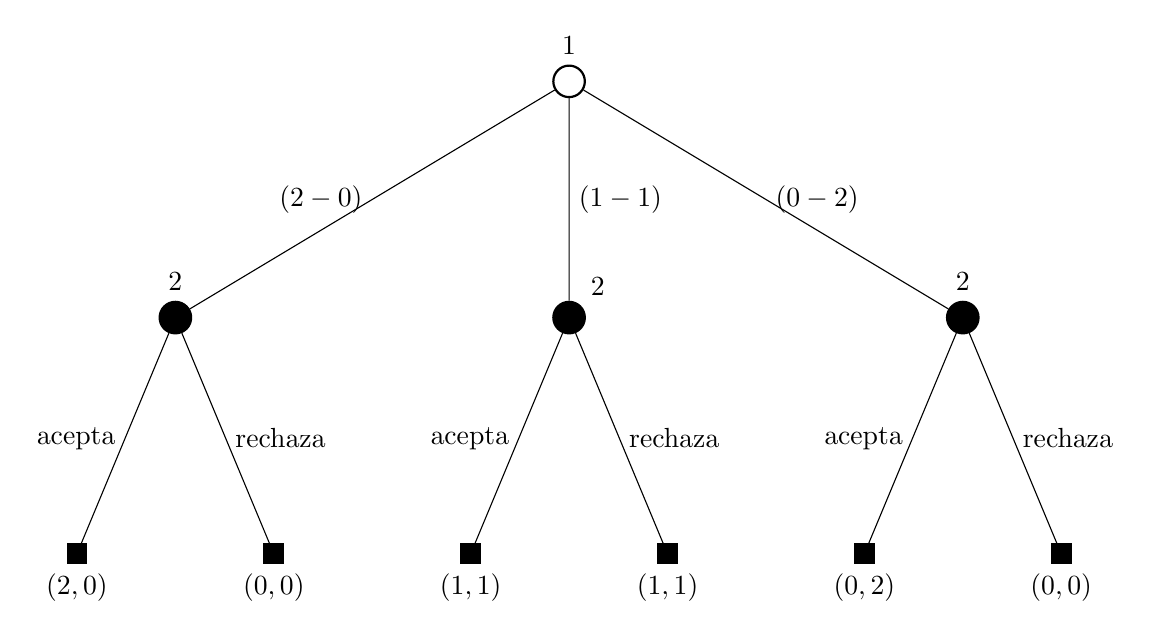
\begin{tikzpicture}[
player1/.style={circle, draw=black, thick, minimum size = 4mm},
player2/.style={circle, draw=black, fill=black, thick, minimum size=4mm},
terminal/.style={rectangle, draw=black, fill=black, thick, minimum size=2mm},
level 1/.style={sibling distance=5cm, level distance=3cm},
level 2/.style={sibling distance=2.5cm},
]
\node[player1] [label=$1$]{}
    child { node [player2] [label=above:{$2$}] {}
    	child { node [terminal] [label=below:{$(2,0)$}] {}
        		edge from parent node[left] {acepta} }
        child { node [terminal] [label=below:{$(0,0)$}] {}
        		edge from parent node[right] {rechaza} }
        edge from parent node[left] {$(2-0)$}
    }
    child { node [player2] [label=45:{$2$}] {}
    	child { node [terminal] [label=below:{$(1,1)$}] {}
        		edge from parent node[left] {acepta} }
        child { node [terminal] [label=below:{$(1,1)$}] {}
        		edge from parent node[right] {rechaza} }
        edge from parent node[right] {$(1-1)$}
    }
    child { node [player2] [label=above:{$2$}] {}
    	child { node [terminal] [label=below:{$(0,2)$}] {}
        		edge from parent node[left] {acepta} }
        child { node [terminal] [label=below:{$(0,0)$}] {}
        		edge from parent node[right] {rechaza} }
        edge from parent node[right] {$(0-2)$}
    };
\end{tikzpicture}
\end{center}
\end{figure}

Sin embargo, es importante diferenciar entre dos tipos de juegos: con información completa (o perfecta) y con información incompleta (o imperfecta). En los juegos con información completa los jugadores tienen toda la información sobre las acciones realizadas previamente de todos los jugadores y del estado actual del juego. El Ejemplo \ref{ex:game-allocation} es un ejemplo de este tipo de juegos; una definición formal es dada en \cite[pp. 89--90]{bib:course-game-theory}.

Por otra parte, en juegos con información incompleta el jugador no tiene toda la información de las acciones tomadas previamente, e incluso pudo haber olvidado las acciones que él u otro jugador realizaron previamente. Por lo cual, un jugador puede no tener suficiente información para determinar en qué nodo del árbol se encuentra. Esto se muestra con el Ejemplo \ref{ex:informacion-incompleta} \cite[p.~202]{bib:course-game-theory}

\begin{example}
\label{ex:informacion-incompleta}
Considere un juego de dos jugadores, el jugador $1$ y el jugador $2$, el cual ocurre como sigue: primero, el jugador $1$ debe elegir una opción entre $L$ y $R$. Si elige $R$ el juego termina; si elige $L$ se le informa al jugador $2$ que el jugador $1$ eligió $L$ y este debe elegir una opción entre $A$ y $B$. Por último, el jugador $1$ debe escoger una nueva opción entre $l$ y $r$, pero sin saber que opción eligió el jugador $2$. Los pagos son mostrados en las hojas del árbol del juego, presentado en la Figura~\ref{fig:informacion-incompleta}
\end{example}

\begin{figure}
\begin{center}
\caption{Árbol del juego en forma extensiva presentado en el Ejemplo~\ref{ex:informacion-incompleta}}
\label{fig:informacion-incompleta}
\begin{tikzpicture}[
player1/.style={circle, draw=black, thick, minimum size = 4mm},
player2/.style={circle, draw=black, fill=black, thick, minimum size=4mm},
terminal/.style={rectangle, draw=black, fill=black, thick, minimum size=2mm},
level 1/.style={sibling distance=6cm, level distance=3cm},
level 2/.style={sibling distance=5cm},
level 3/.style={sibling distance=2.5cm, level distance=2cm},
]
\node[player1] [label=$1$] {}
	child { node [player2] [label=above:{$2$}]  {}
    	child { node (A) [player1] [label=left:{$1$}]  {} 
        		child { node [terminal] [label=below:{$(0,0)$}] {} 
                		edge from parent node[left] {$l$} }
                child { node [terminal] [label=below:{$(2,4)$}] {}
                		edge from parent node[right] {$r$}}
                edge from parent node[left] {A}
        }
        child { node (B) [player1] [label=right:{$1$}] {}
        		child { node [terminal] [label=below:{$(2,4)$}] {}
                		edge from parent node[left] {$l$} }
                child { node [terminal] [label=below:{$(0,0)$}] {} 
                		edge from parent node[right] {$r$} }
                edge from parent node[right] {B}
        }
        edge from parent node[left] {L}
    }
    child { node [terminal] [label=below:{$(1,1)$}] {}
    		edge from parent node[right] {R} };
\draw[dotted] (A) -- (B);
\end{tikzpicture}
\end{center}
\end{figure}

Se puede observar que los nodos unidos por líneas punteadas son indistinguibles para el jugador $1$, pues él no sabe cuál fue la elección del jugador $2$. Este tipo de nodos originan los llamados \textbf{conjuntos de información}, definidos formalmente en la Definición~\ref{def:informacion-incompleta} \cite[p.~200]{bib:course-game-theory}. Esta definición no incluye los árboles del juego de forma explícita. En cambio utiliza secuencias de acciones, que serán equivalentes a los caminos desde la raíz hasta los nodos del árbol. Una definición basada en el árbol del juego puede ser encontrada en \cite{bib:conceptos-basicos}.

\begin{definition}
\label{def:informacion-incompleta}
Un juego finito en \textbf{forma extensiva} con \textbf{información incompleta} tiene los siguientes componentes:
\begin{itemize}[noitemsep]
  \item Un conjunto finito $N$ de \textbf{jugadores}.
  \item Un conjunto finito $H$ de secuencias, las posible \textbf{historias} de acciones, tal que la secuencia vacía está en $H$, y cada prefijo de una secuencia en $H$ también está en $H$. $Z \subseteq H$ son las historias terminales (aquellas que no son prefijo de ninguna otra secuencia). $A(h) = \{ a : (h, a) \in H \}$ son las acciones disponibles después de una historia no terminal $h \in H$.
  \item Una función $P$ que asigna a cada historia no terminal (cada elemento de $H \setminus Z)$ un elemento de $N \cup \{c \}$. $P$ es la \textbf{función de jugador}. $P(h)$ es el jugador que toma una acción después de la historia $h$. Si $P(h) = c$ entonces la acción tomada después de la historia $h$ es determinada por el azar. Este tipo de nodos serán denominados \textbf{nodos de azar}.
  \item Una función $f_c$ que asocia con cada historia $h$ para la cual $P(h) = c$ una medida de probabilidad $f_c(.|h)$ sobre $A(h)$: $f_c(a|h)$ es la probabilidad que la acción $a$ ocurra dado $h$.  Cada medida de probabilidad es independiente de cualquier otra de estas medidas.
  \item Para cada jugador $i \in N$, una partición $\mathcal{I}_i$ de $\{h \in H : P(h) = i\}$ con la propiedad que $A(h) = A(h')$ siempre que $h$ y $h'$ estén en el mismo bloque de la partición. Para $I_i \in \mathcal{I}_i$ denotamos por $A(I_i)$ el conjunto $A(h)$ y por $P(I_i)$ el jugador $P(h)$ para cualquier $h \in I_i$. $\mathcal{I}_i$ es la \textbf{partición de información} del jugador $i$, un conjunto $I_i \in \mathcal{I}_i$ es un \textbf{conjunto de información} del jugador $i$.
  \item Para cada jugador $i \in N$, una función de utilidad $u_i$ de los estados terminales $Z$ a los reales $\mathbb{R}$. Si $N = \{1,2\}$ y $u_1 = -u_2$, decimos que tenemos un \textbf{juego de dos jugadores de suma cero en forma extensiva}. Definamos $\Delta_{u,i} = \max_z u_i(z) - \min_z u_i(z)$ como el rango de utilidades del jugador $i$.
\end{itemize}
\end{definition}

En el Ejemplo \ref{ex:informacion-incompleta}, $H = \{ \emptyset, L, R, LA, LB, LAl, LAr, LBl, LBr\}$, note que la cantidad de elementos en $H$ coincide con la cantidad de nodos del árbol. En efecto, en un árbol para cualquier nodo $u$ existe un camino único desde la raíz hasta $u$. Además, $P(\emptyset) = P(LA) = P(LB) = 1$, y $P(L) = 2$. Las particiones de información son $\mathcal{I}_1 = \{\{\emptyset\}, \{LA, LB\}\}$ y $\mathcal{I}_2  = \{\{L\}\}$. En la definición se incluye un elemento que no está presente en el ejemplo, los \textbf{nodos de azar}. Estos nodos corresponden a acciones que no dependen de los jugadores, sino de algún evento externo aleatorio, como el lanzamiento de una moneda, lanzamiento de uno o más dados, o la repartición de cartas en un juego.

\subsection{Juego de Kuhn Poker}
\label{section:kuhn-poker}

Kuhn Poker es una versión simplificada del juego de Poker con tres cartas y dos jugadores (denominados jugador $1$ y jugador $2$) definido por Harold W.\ Kuhn \cite{bib:kuhn-poker}. En este juego se barajan tres cartas marcadas con los números $1$, $2$ y $3$. Posteriormente, cada jugador recibe una de ellas, manteniendo su número como información privada. Es decir, un jugador sabe su propio número pero no sabe el número de su oponente. Al inicio del juego cada jugador apuesta una ficha. El juego ocurre por turnos, los cuales se alternan entre los jugadores comenzando por el jugador $1$. En un turno un jugador puede \textit{apostar} o \textit{pasar}. Si un jugador apuesta debe apostar una ficha adicional. Si un jugador pasa después de una apuesta, el oponente gana y toma todas las fichas apostadas. Si hay dos apuestas o dos pases seguidos los jugadores muestran sus cartas y gana el jugador con el número más alto obteniendo todas las fichas apostadas. La Tabla \ref{table:kunh-poker} presenta un resumen de todas las posibles secuencias con su respectivo pago a cada jugador.

\begin{table}[ht]
\begin{center}
\caption[Resumen de las posibles secuencias del juego Kunh Poker]{Resumen de las posibles secuencias del juego Kunh Poker}
\label{table:kunh-poker}
\begin{tabular}{ | c | c | c | c |}
\multicolumn{3}{c}{Secuencia de Acciones} & \multicolumn{1}{c}{\empty} \\ \hline
Jugador $1$ & Jugador $2$ & Jugador $1$ & Pago \\ \hline
\multirow{3}{*}{pasar} & pasar & & $+1$ al jugador con la carta más alta\\
& apostar & pasar & $+1$ al jugador $2$\\
& apostar & apostar & $+2$ al jugador con la carta más alta \\ \hline
\multirow{2}{*}{apostar} & pasar & & $+1$ al jugador $1$ \\
& apostar & &  $+2$ al jugador con la carta más alta \\ \hline
\end{tabular}
\end{center}
\end{table}

Debido a qué es un juego de suma $0$, el jugador perdedor pierde el número de fichas que gana su oponente. El árbol del juego se muestra en la Figura \ref{fig:kunh-poker}. La raíz es un \textit{nodo de azar}, que representa la repartición de las cartas, con $6$ opciones diferentes, las cuales están representadas con un par ordenado indicando la carta del jugador $1$ y la del jugador $2$. Cada rama tiene una probabilidad de $\frac{1}{6}$ de ser elegida. Los nodos del primer nivel y tercer nivel corresponden al jugador $1$. Este jugador tiene $6$ conjuntos de información diferentes, cada uno con $2$ nodos, los cuales se unen mediante las líneas punteadas. Los nodos del segundo nivel corresponden al jugador $2$, los conjuntos de información se representan por nodos del mismo color y mismo estilo (relleno de color o no). En cada nodo de decisión (los nodos no terminales sin incluir la raíz), hay dos opciones: pasar, representado con una línea punteada, o apostar, representado con una línea doble. Los nodos terminales tienen la ganancia del jugador $1$, según sea el caso.

\begin{figure}
\begin{center}
\caption{Árbol completo del juego Kunh Poker.}
\label{fig:kunh-poker}
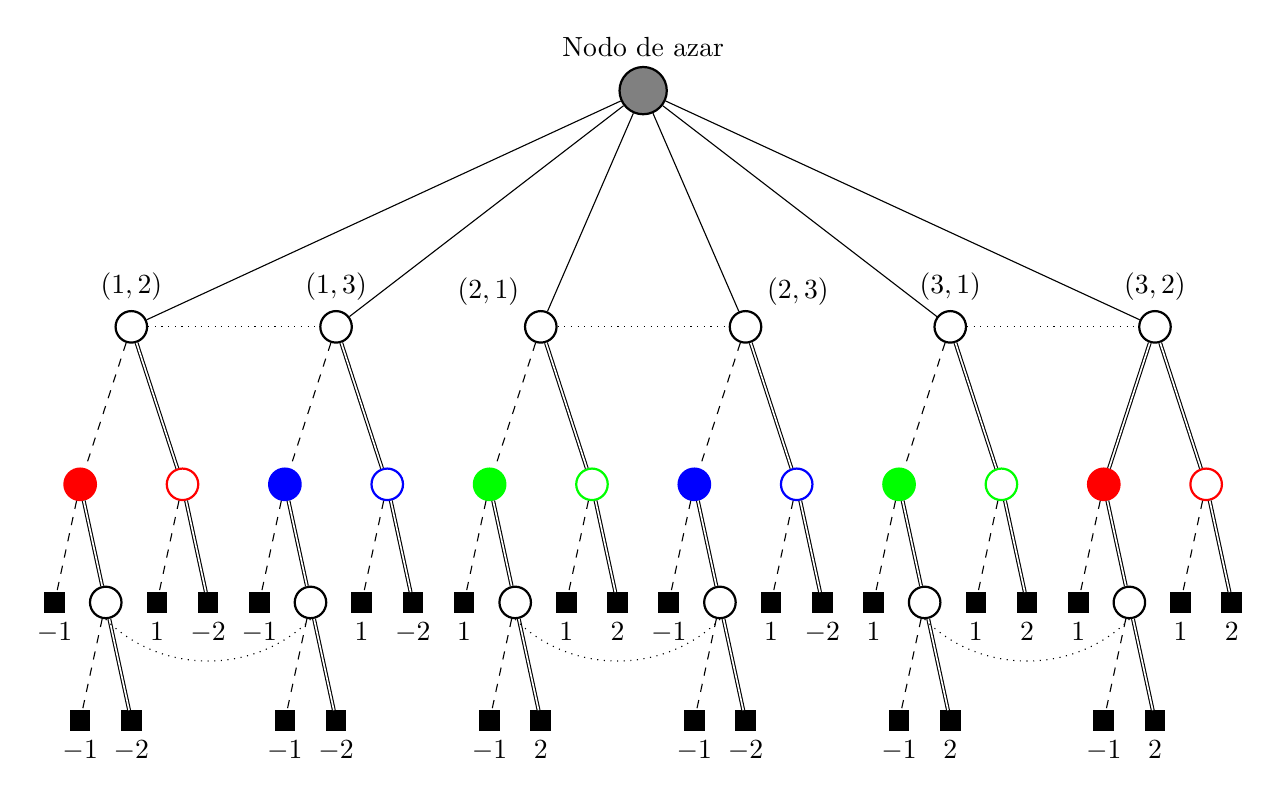
\begin{tikzpicture}[
chance/.style={circle, draw=black, fill=gray, thick, minimum size = 6mm},
player1/.style={circle, draw=black, solid, thick, minimum size = 4mm},
player2/.style={circle, thick, minimum size=4mm},
terminal/.style={rectangle, draw=black, solid, fill=black, thick, minimum size=2mm},
level 1/.style={sibling distance=26mm, level distance=30mm},
level 2/.style={sibling distance=13mm, level distance=20mm},
level 3/.style={sibling distance=6.5mm, level distance=15mm},
]
\node[chance] [label=above:{Nodo de azar}] {} {
	child {node [player1] (P1) [label=above:{$(1, 2)$}]{}
		child { node [player2] [draw=red, fill=red] {} 
				child { node [terminal] [label=below:{$-1$}] {}
						edge from parent [dashed] {} }
				child { node [player1] (A) {} 
						child { node [terminal] [label=below:{$-1$}] {}
								edge from parent [dashed] {} }
						child { node [terminal] [label=below:{$-2$}] {} 
								edge from parent [solid, double] {} }
						edge from parent [solid, double] {}
				}
				edge from parent [dashed] {}
		}
		child { node [player2] [draw=red] {} 
				child { node [terminal] [label=below:{$1$}] {}
						edge from parent [dashed] {} }
				child { node [terminal] [label=below:{$-2$}] {}
						edge from parent [solid, double] {} }
				edge from parent [solid, double] {}
		}
	}
	child {node [player1] (P2) [label=above:{$(1, 3)$}]{}
		child { node [player2] [draw=blue, fill=blue] {} 
				child { node [terminal] [label=below:{$-1$}] {}
						edge from parent [dashed] {} }
				child { node [player1] (B) {} 
						child { node [terminal] [label=below:{$-1$}] {}
								edge from parent [dashed] {} }
						child { node [terminal] [label=below:{$-2$}] {}
								edge from parent [solid, double] {} }
						edge from parent [solid, double] {}
				}
				edge from parent [dashed] {}
		}
		child { node [player2] [draw=blue] {} 
				child { node [terminal] [label=below:{$1$}] {}
						edge from parent [dashed] {} }
				child { node [terminal] [label=below:{$-2$}] {}
						edge from parent [solid, double] {} }
				edge from parent [solid, double] {}
		}
	}
	child {node [player1] (P3) [label=135:{$(2, 1)$}]{}
		child { node [player2] [draw=green, fill=green] {} 
				child { node [terminal] [label=below:{$1$}] {}
						edge from parent [dashed] {} }
				child { node [player1] (C) {} 
						child { node [terminal] [label=below:{$-1$}] {}
								edge from parent [dashed] {} }
						child { node [terminal] [label=below:{$2$}] {}
								edge from parent [solid, double] {} }
						edge from parent [solid, double] {}
				}
				edge from parent [dashed] {}
		}
		child { node [player2] [draw=green] {} 
				child { node [terminal] [label=below:{$1$}] {}
						edge from parent [dashed] {} }
				child { node [terminal] [label=below:{$2$}] {}
						edge from parent [solid, double] {} }
				edge from parent [solid, double] {}
		}
	}
	child {node [player1] (P4) [label=45:{$(2, 3)$}]{}
		child { node [player2] [draw=blue, fill=blue]{} 
				child { node [terminal] [label=below:{$-1$}] {}
						edge from parent [dashed] {} }
				child { node [player1] (D) {} 
						child { node [terminal] [label=below:{$-1$}] {}
								edge from parent  [dashed] {} }
						child { node [terminal] [label=below:{$-2$}] {}
								edge from parent [solid, double] {} }
						edge from parent [solid, double] {}
				}
				edge from parent [dashed] {}
		}
		child { node [player2] [draw=blue] {} 
				child { node [terminal] [label=below:{$1$}] {}
						edge from parent [dashed] {} }
				child { node [terminal] [label=below:{$-2$}] {}
						edge from parent [solid, double] {} }
				edge from parent [solid, double] {}
		}
	}
	child {node [player1] (P5) [label=above:{$(3, 1)$}]{}
		child { node [player2] [draw=green, fill=green] {} 
				child { node [terminal] [label=below:{$1$}] {}
						edge from parent [dashed] {} }
				child { node [player1] (E) {} 
						child { node [terminal] [label=below:{$-1$}] {}
								edge from parent [dashed] {} }
						child { node [terminal] [label=below:{$2$}] {}
								edge from parent [solid, double] {} }
						edge from parent [solid, double] {}
				}
				edge from parent [dashed] {}
		}
		child { node [player2] [draw=green] {} 
				child { node [terminal] [label=below:{$1$}] {}
						edge from parent [dashed] {} }
				child { node [terminal] [label=below:{$2$}] {}
						edge from parent [solid, double] {} }
				edge from parent [solid, double] {}
		}
	}
	child {node [player1] (P6) [label=above:{$(3, 2)$}]{}
		child { node [player2]  [draw=red, fill=red] {} 
				child { node [terminal] [label=below:{$1$}] {}
						edge from parent [dashed] {} }
				child { node [player1] (F) {} 
						child { node [terminal] [label=below:{$-1$}] {}
								edge from parent [dashed] {}}
						child { node [terminal] [label=below:{$2$}] {}
								edge from parent [solid, double] {} }
						edge from parent [solid, double] {}
				}
				edge from parent [solid, double] {}
		}
		child { node [player2]  [draw=red] {} 
				child { node [terminal] [label=below:{$1$}] {}
						edge from parent [dashed] {} }
				child { node [terminal] [label=below:{$2$}] {}
						edge from parent [solid, double] {} }
				edge from parent [solid, double] {}
		}
	}
};
\draw[dotted]
(A.south) .. controls ++(-45:10mm) and ++(45:-10mm) .. (B.south);
\draw[dotted]
(C.south) .. controls ++(-45:10mm) and ++(45:-10mm) .. (D.south);
\draw[dotted]
(E.south) .. controls ++(-45:10mm) and ++(45:-10mm) .. (F.south);
\draw[dotted] (P1.east) -- (P2.west);
\draw[dotted] (P3.east) -- (P4.west);
\draw[dotted] (P5.east) -- (P6.west);
\end{tikzpicture}
\end{center}
\end{figure}

\subsection{Estrategias Puras y Mixtas para Juegos en Forma Extensiva}

Al igual que en juegos en forma normal es necesario establecer las definiciones de estrategias. Las Definiciones \ref{def:estrategia-pura-fe} y \ref{def:estrategia-mixta-fe}, presentan los conceptos de estrategia pura y estrategia mixta, análogas a las presentadas en los juegos en forma normal. Las definiciones de perfiles estratégicos son equivalentes a las anteriores pero usando los conceptos de estrategias de esta sección. Además, se procura utilizar una notación similar a la utilizada en la sección anterior. Sin embargo, se presenta un nuevo concepto, las \textbf{estrategias de comportamiento}, que son exclusivas para juegos en forma extensiva. Los conceptos presentados están basados en las definiciones de \cite{bib:conceptos-basicos} y \cite{bib:course-game-theory}.

\begin{definition}
\label{def:estrategia-pura-fe}
Una \textbf{estrategia pura} para el jugador $i$ es una función $s_i : \mathcal{I}_i \rightarrow \bigcup_{I_i \in \mathcal{I}_i}A(I_i)$ tal que $s_i(I_i) \in A(I_i)$, donde $A(I_i) = A(h)$ para cualquier $h \in I_i$. 
\end{definition}

Note que una estrategia pura consiste en elegir una acción por cada conjunto de información de un jugador en específico. Considere nuevamente el Ejemplo \ref{ex:informacion-incompleta}. En este juego el jugador $1$ tiene dos conjuntos de información, $I^1 = \{\emptyset\}$ e $I^2 = \{LA, LB\}$, cada uno con dos posibles elecciones, dando lugar a $4$ estrategias puras que son denotadas por $s_1$, $s_2$, $s_3$ y $s_4$, y presentadas en la Tabla~\ref{table:estrategias-puras}. En dicha tabla las acciones posibles en el conjunto de información $I^1$ están representadas por las filas, y las acciones en $I^2$ por las columnas. De esta forma cada celda representa una única estrategia pura determinada por una acción en cada conjunto de información.

\begin{table}[ht]
\begin{center}
\caption{Estrategias puras para el juego con información incompleta presentado en el Ejemplo \ref{ex:informacion-incompleta}.}
\label{table:estrategias-puras}
\begin{tabular}{c c | c | c | }
 &  \multicolumn{1}{c}{} & \multicolumn{2}{c}{$I_2$} \\
 &  \multicolumn{1}{c | }{} & \multicolumn{1}{c | }{l} & r \\ \cline{2-4}
 \multirow{2}{*}{$I_1$} & $L$ & $s_1=$  elegir L y l & $s_2=$ elegir L y r\\ \cline{2-4}
 & $R$ & $s_3=$ elegir R y l & $s_4=$ elegir R y r \\ \cline{2-4}
\end{tabular}
\end{center}
\end{table}

En Kunh Poker una estrategia pura para el jugador $2$ puede ser la siguiente: si su carta contiene el número $1$ siempre pasa, si su carta contiene el número $2$ apuesta si y sólo si el jugador $1$ pasa en su primer turno, y si su carta contiene el número $3$ siempre apuesta. La Tabla \ref{table:ejemplo-estrategia-pura} presenta cada conjunto de información de forma explícita con su acción correspondiente. Para este juego se caracterizarán los conjuntos de información del jugador $2$ por la carta que tiene y la acción realizada por el primer jugador al inicio del juego.

\begin{table}[ht]
\begin{center}
\caption{Ejemplo de una estrategia pura para el jugador $2$ en el juego Kunh Poker.}
\label{table:ejemplo-estrategia-pura}
\begin{tabular}{ c c | c }
\hline
\multicolumn{2}{c | }{Conjunto de Información} & \multirow{2}{*}{Acción del jugador $2$} \\ 
Carta del jugador $2$ & Acción del jugador $1$ &  \\ \hline
$1$ & pasar & pasar \\
$1$ & apostar & pasar \\
$2$ & pasar & apostar \\
$2$ & apostar & pasar \\
$3$ & pasar & apostar \\
$3$ & apostar & apostar \\
\hline
\end{tabular}
\end{center}
\end{table}

Se denotará, al igual que en los juegos en forma normal, con $S_i$ al conjunto de estrategias puras del jugador $i$, es decir $S_i=\prod_{I_i \in \mathcal{I}_i} A(I_i)$. Análogamente, se denotará con $S = \prod_{i \in N} S_i$ el conjunto de todas las estrategias puras de todos los jugadores de forma simultánea. Un elemento $s \in S$ es llamado un \textbf{perfil estratégico}.

Otra definición de interés es la función de pago para una estrategia pura. Para esto se denotará con $\pi^s(h)$ la probabilidad que $h \in H $ ocurra si todos los jugadores juegan con la estrategia $s$. Luego, definimos $u_i : S \rightarrow \mathbb{R}$ como la esperanza de la función de pago para el jugador $i$ para cada perfil estratégico, la cual viene dada por:
\begin{alignat}{1}
\label{eq:funcion-pago-fe}
u_i(s)\ =\ \sum_{z \in Z} \pi^s(z) u_i(z) \,.
\end{alignat} 

\begin{definition}
\label{def:estrategia-mixta-fe}
Una \textbf{estrategia mixta} $\sigma^m_i$ para el jugador $i$ es una distribución de probabilidad sobre $S_i$. Es decir, $\sigma_i^m \in \Delta(S_i)$.
\end{definition}

\begin{definition}
Una \textbf{perfil estratégico mixto} $\sigma^m \in \prod_{i \in N} \Delta(S_i)$ consiste en una estrategia mixta para cada jugador de forma $\sigma^m = (\sigma_1^m, \sigma_2^m, ...., \sigma_N^m)$.
\end{definition}

Un perfil estratégico mixto indica que cada jugador elige, antes de que el juego comience, un plan completo (es decir, una estrategia pura) de forma aleatoria acorde a cierta distribución de probabilidad (que está dada por su estrategia mixta respectiva).

Si $\sigma^m \in \prod_{i = 1}^N \Delta(S_i)$ es un perfil estratégico mixto, la ganancia esperada del jugador $i$, cuando todos los jugadores juegan acorde a $\sigma^m$ viene dada por:
\begin{alignat}{1}
u_i(\sigma^m)\ =\ \sum_{s \in S} \sigma^m(s)u_i(s)
\end{alignat}
donde $\sigma^m(s)$ es la probabilidad de que $s$ sea elegida, es decir $\sigma^m(s) = \prod_{i \in N} \sigma_i^m(s_i)$.

\subsection{Forma Normal y Forma Extensiva de un Juego}
\label{section:normal-extensiva}

Un juego en forma normal %(Definición \ref{def:forma-normal})
se caracteriza por el conjunto de estrategias puras $S_i$ y la función de pago $u_i$ para cada jugador $i\in N$. Estos elementos pueden obtenerse a partir de la descripción de un juego en forma extensiva utilizando las definiciones \ref{def:estrategia-pura-fe} y \ref{eq:funcion-pago-fe}. De esta forma, es posible asociar un único juego en forma normal a cualquier juego en forma extensiva.

En el Ejemplo \ref{ex:informacion-incompleta}, las estrategias puras para el jugador $1$ están definidas en la Tabla \ref{table:estrategias-puras}. El jugador dos tiene sólo dos estrategias puras, elegir $A$ o $B$. Luego, la Tabla \ref{table:fextensiva-a-fnormal} es la tabla de pagos para juego en forma normal que corresponde al Ejemplo \ref{ex:informacion-incompleta}.

\begin{table}[ht]
\begin{center}
\caption[Forma normal de un juego en forma extensiva]{Tabla de pagos de la forma normal correspondiente a la forma extensiva del juego presentado en el Ejemplo \ref{ex:informacion-incompleta}.}
\label{table:fextensiva-a-fnormal}
\begin{tabular}{ c | c  c }
\hline
\multicolumn{1}{c}{} & \multicolumn{2}{|c}{Jugador $2$} \\ 
Jugador $1$ & \multicolumn{1}{c}{ Elegir $A$ } & Elegir $B$ \\ \hline
Elegir $L$ y $l$ & $0,0$ & $2,4$ \\
Elegir $L$ y $r$ & $2,4$ & $0,0$ \\
Elegir $R$ y $l$ & $1,1$ & $1,1$ \\
Elegir $R$ y $r$ & $1,1$ & $1,1$ \\ \hline
\end{tabular}
\end{center}
\end{table}

Note que la tabla obtenida tiene $8$ configuraciones a pesar que el árbol original tiene sólamente $5$ nodos terminales. En general, la forma normal tiene un tamaño exponencial en el tamaño del árbol del juego en forma extensiva. Se observa que más de una celda (o una estrategia pura) lleva al mismo nodo terminal. Esto ocurre cuando el primer jugador elige $R$, en este caso no importa la segunda elección del primer jugador, ni la estrategia utilizada por el segundo jugador, pues el juego siempre terminará luego que el jugador $1$ elija $R$. Por esto la forma normal de un juego es potencialmente más grande que su forma extensiva.

Por otra parte, dado un juego en forma normal, siempre es posible construir el árbol de una forma extensiva como sigue \cite{bib:conceptos-basicos}: se comienza por la raíz, la cual es el único nodo del jugador $1$, de ésta salen $|S_1|$ ramas, una para cada estrategia pura $s_1 \in S_1$, estos nodos, los hijos de la raíz, serán los nodos del jugador $2$. De cada uno de los nodos del jugador $2$ salen $|S_2|$ ramas, una por cada elemento $s_2 \in S_2$ que serán los hijos del jugador $3$, y así sucesivamente hasta llegar a los hijos de los nodos del jugador $N$, que serán los nodos terminales. La Figura \ref{fig:RPS}, muestra el árbol para una forma extensiva del juego piedra (R), papel (P) o tijera (S).

\begin{figure}
\begin{center}
\caption{Árbol de la forma extensiva del juego \textit{Piedra, Papel o Tijeras}}
\label{fig:RPS}
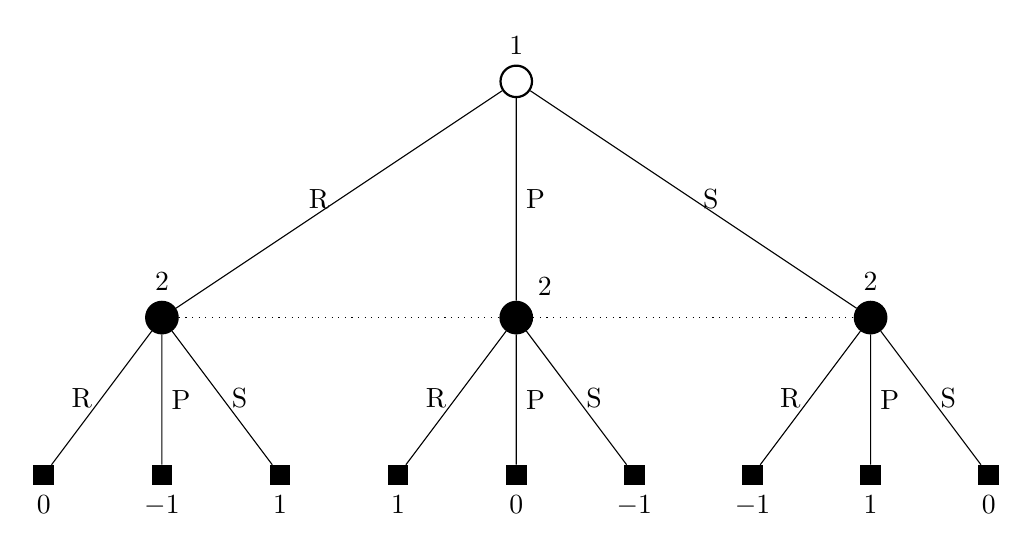
\begin{tikzpicture}[
chance/.style={circle, draw=black, fill=black, thick, minimum size = 6mm},
player1/.style={circle, draw=black, thick, minimum size = 4mm},
player2/.style={circle, draw=black, fill=black, thick, minimum size=4mm},
terminal/.style={rectangle, draw=black, fill=black, thick, minimum size=2mm},
level 1/.style={sibling distance=45mm, level distance=3cm},
level 2/.style={sibling distance=15mm, level distance=20mm},
]
\node[player1] [label=$1$] {}
	child { node (A) [player2] [label=above:{$2$}]  {}
    	child { node [terminal] [label=below:{$0$}] {}
        		edge from parent node[left] {R} }
        child { node [terminal] [label=below:{$-1$}] {}
        		edge from parent node[right] {P} }
        child { node [terminal] [label=below:{$1$}] {}
        		edge from parent node[right] {S} }
    edge from parent node[left] {R}
    }
    child { node (B) [player2] [label=45:{$2$}] {}
    	child { node [terminal] [label=below:{$1$}] {}
        		edge from parent node[left] {R} }
        child { node [terminal] [label=below:{$0$}] {}
        		edge from parent node[right] {P} }
        child { node [terminal] [label=below:{$-1$}] {}
        		edge from parent node[right] {S} }
    edge from parent node[right] {P}
    }
    child { node (C) [player2] [label=above:{$2$}] {}
    	child { node [terminal] [label=below:{$-1$}] {}
        		edge from parent node[left] {R} }
        child { node [terminal] [label=below:{$1$}] {}
        		edge from parent node[right] {P} }
        child { node [terminal] [label=below:{$0$}] {}
        		edge from parent node[right] {S} }
    edge from parent node[right] {S}
    };
\draw[dotted] (A) -- (B) -- (C);
\end{tikzpicture}
\end{center}
\end{figure}

Pueden haber diferentes formas extensivas que lleven a la misma forma normal. En efecto, si aplicamos el procedimiento descrito anteriormente a la Tabla \ref{table:fextensiva-a-fnormal} se obtiene un árbol de $13$ nodos  (Figura \ref{fig:arbol-de-tabla}), en contraste a los $9$ nodos del árbol original. En efecto, la forma extensiva proporciona más información sobre los juegos que la forma normal. En especial, la forma extensiva proporciona información acerca del orden y las posibles secuencias de acciones.

\begin{figure}
\begin{center}
\caption{Árbol correspondiente a la forma normal de la Tabla \ref{table:fextensiva-a-fnormal}}
\label{fig:arbol-de-tabla}
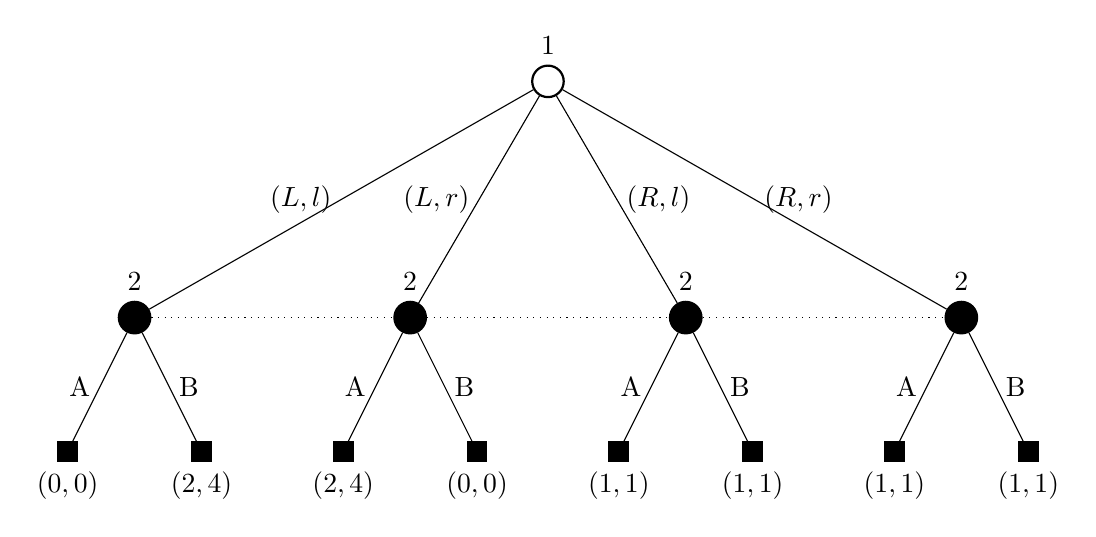
\begin{tikzpicture}[
chance/.style={circle, draw=black, fill=black, thick, minimum size = 6mm},
player1/.style={circle, draw=black, thick, minimum size = 4mm},
player2/.style={circle, draw=black, fill=black, thick, minimum size=4mm},
terminal/.style={rectangle, draw=black, fill=black, thick, minimum size=2mm},
level 1/.style={sibling distance=35mm, level distance=3cm},
level 2/.style={sibling distance=17mm, level distance=17mm},
]
\node[player1] [label=$1$] {}
	child { node (A) [player2] [label=above:{$2$}]  {}
    	child { node [terminal] [label=below:{$(0,0)$}] {}
        		edge from parent node[left] {A} }
        child { node [terminal] [label=below:{$(2,4)$}] {}
        		edge from parent node[right] {B} }
        edge from parent node[left] {$(L, l)$}
    }
    child { node (B) [player2] [label=above:{$2$}] {}
    	child { node [terminal] [label=below:{$(2,4)$}] {}
        		edge from parent node[left] {A} }
        child { node [terminal] [label=below:{$(0,0)$}] {}
        		edge from parent node[right] {B} }
        edge from parent node[left] {$(L, r)$}
    }
    child { node (C) [player2] [label=above:{$2$}] {}
    	child { node [terminal] [label=below:{$(1,1)$}] {}
        		edge from parent node[left] {A} }
        child { node [terminal] [label=below:{$(1,1)$}] {}
        		edge from parent node[right] {B} }
        edge from parent node[right] {$(R, l)$}
    }
    child { node (D) [player2] [label=above:{$2$}] {}
    	child { node [terminal] [label=below:{$(1,1)$}] {}
        		edge from parent node[left] {A} }
        child { node [terminal] [label=below:{$(1,1)$}] {}
        		edge from parent node[right] {B} }
        edge from parent node[right] {$(R, r)$}
    };
\draw[dotted] (A) -- (B) -- (C) -- (D);
\end{tikzpicture}
\end{center}
\end{figure}

\subsection{Estrategias de Comportamiento}

En juegos en forma extensiva, el jugador puede utilizar un tipo de estrategia diferente a la presentada anteriormente, y la cual es denominada estrategia de comportamiento (Definición \ref{def:estrategia-comportamiento}). Una estrategia de comportamiento para el jugador $i$ especifica una distribución de probabilidad sobre las acciones disponibles en cada conjunto de información del jugador $i$. Esto difiere a las estrategias mixtas que representan una distribución de probabilidad sobre las estrategias puras de un jugador \cite[p. 212]{bib:course-game-theory}. 

\begin{definition}
\label{def:estrategia-comportamiento}
Una \textbf{estrategia de comportamiento} para el jugador $i$ consiste en una distribución de probabilidad para cada conjunto de información $I_i \in \mathcal{I}_i$ sobre el conjunto $A(I_i)$ que pueden ejecutarse en $I_i$.
Es decir, una estrategia de comportamiento es una tupla $(\sigma^b_i(I_i))_{I_i \in \mathcal{I}_i}$ donde $\sigma^b_i(I_i) \in \Delta(A(I_i))$.
\end{definition}

Sea $B^i = \prod_{I_i \in \mathcal{I}_i} \Delta(A(I_i))$ el conjunto de todas las posibles estrategias de comportamiento del jugador $i$. Si $\sigma_i^b \in B^i$, $\sigma_i^b(I_i) \in \Delta(A(I_i))$ es una distribución de probabilidad sobre $A(I_i)$ mientras que $\sigma_i^b(I_i)(a)$ es la probabilidad de elegir la acción $a$ dada una historia $h \in I_i$.

\begin{definition}
Una \textbf{perfil estratégico de comportamiento} $\sigma^b$ es una estrategia de comportamiento para cada jugador.
\end{definition}

El conjunto de todos los perfiles estratégicos de comportamiento es $B = \prod_{i \in N} B^i$. Si $\sigma^b \in B$, la utilidad esperada de la estrategia $\sigma^b$ para el jugador $i$ es
\[ u_i(\sigma^b)\ =\ \sum_{s \in S} \sigma_b(s)u_i(s) \]
donde $\sigma_i^b(s_i) = \prod_{I_i \in \mathcal{I}_i} \sigma_i^b(I_i)(s_i(I_i))$, y $\sigma^b(s) =  \prod_{i \in N} \sigma_i^b(s_i)$.

Con las definiciones proporcionadas se puede definir los conceptos de equilibrio de Nash y aproximación de equilibrio de Nash para juegos en forma extensiva.

\begin{definition}
Sea $\Sigma=\prod_{i\in N}\Sigma_i$ el conjunto de perfiles mixtos o de comportamiento, según sea el caso, para los jugadores en $N$.
Para $\varepsilon\geq 0$, decimos que un perfil estratégico $\sigma \in \Sigma$ es un \textbf{$\varepsilon$-equilibrio de Nash} si y sólo si para todo jugador $i$ y perfil $\sigma'_i\in\Sigma_i$,
\begin{alignat}{1}
u_i(\sigma) + \varepsilon\ \geq\ u_i(\sigma'_i, \sigma_{-i}) \,.
\end{alignat}
El perfil $\sigma\in\Sigma$ es un \textbf{equilibrio de Nash} si y sólo si $\sigma$ es un $0$-equilibrio de Nash.
\end{definition}

En el Ejemplo~\ref{ex:informacion-incompleta} se tienen $4$ estrategias puras para el jugador $1$ (Tabla \ref{table:estrategias-puras}). Una estrategia mixta $\sigma^m_1$ es una distribución de probabilidad sobre el conjunto $\{s_1, s_2, s_3, s_4\}$, donde las probabilidades son $\sigma^m_1(s_1)$, $\sigma^m_1(s_2)$, $\sigma^m_1(s_3)$ y $\sigma^m_1(s_4)$. Por otra parte una estrategia de comportamiento $\sigma^b_1$ son dos distribuciones de probabilidad, $\sigma^b_1(I^1)$ y $\sigma^b_1(I_2)$, sobre los conjuntos $A(I^1) = \{L, R\}$ y $A(I^2) = \{l, r\}$ respectivamente.

Sea $\sigma$ un perfil estratégico mixto o de comportamiento. Sea  $\sigma_{-i} = (\sigma_j)_{j \neq i}$ la combinación de todas las estrategias de $\sigma$ excepto $\sigma_i$. Sea $\pi^{\sigma_i}(h)$ la probabilidad de alcanzar $h$ dado que el jugador $i$ utiliza la estrategia $\sigma_i$ y que los demás jugadores juegan para alcanzar $h$. Note que $\pi^{\sigma_i}(h)$ es la probabilidad de que para todo prefijo propio $h' \sqsubset h$ tal que $P(h') = i$, el $i$-ésimo jugador elija la acción $a$ correspondiente en $h$; i.e., $(h', a) \sqsubseteq h$.

Sea $\pi^c(h)$ la probabilidad de alcanzar $h$ asumiendo que todos los jugadores juegan para alcanzar $h$, es decir:
\begin{alignat}{1}
\pi^c(h) = \prod_{(h', a) \sqsubset h : P(h') = c} f_c(a | h') \, .
\end{alignat}

Sea $\pi^{\sigma}(h) = \prod_{i \in N \cup {c}} \pi^{\sigma_i}(h)$ la probabilidad de que la historia $h$ ocurra si todos los jugadores eligen las acciones acorde al perfil estratégico  $\sigma$.  Sea $\pi^{\sigma_{-i}}(h) = \frac{\pi^{\sigma}(h)}{\pi^{\sigma_{i}}(h)}$ el producto de todas las contribuciones de los jugadores (incluyendo las elecciones en las historias de azar) excepto el jugador $i$. Sean $\pi^{\sigma}(I) = \sum_{h \in I},  \pi^\sigma(h)$, $\pi^{\sigma_i}(I) = \sum_{h \in I},  \pi^{\sigma_i}(h)$ y $\pi^{\sigma_{-i}}(h) = \sum_{h \in I},  \pi^{\sigma_{-i}}(h)$ la probabilidad de alcanzar el conjunto de información $I$ dado la estrategia $\sigma$, $\sigma_{i}$ y $\sigma_{-i}$, respectivamente.

Para un perfil estratégico $\sigma$, sea $u_i(\sigma) = \sum_{z \in Z} u_i(z)\pi^{\sigma}(z)$ la ganancia esperada del jugador $i$ cuando todos los jugadores utilizan el perfil estratégico $\sigma$. Sea $I(h)$ el conjunto de información al que pertenece $h$, como los conjuntos de información son una partición de las historias correspondientes a cada jugador $I(h)$ está bien definida. La notación presentada es la utilizada en \cite{bib:cfr}.

\subsection{Perfect Recall}

El concepto de \textit{perfect recall} hace referencia a juegos en los cuales, en cualquier punto cualquier jugador \textit{recuerda} lo que sabía previamente \cite[p.~203]{bib:course-game-theory}. En particular, cada jugador recuerda los movimientos que hizo previamente. La definición de \textit{perfect recall} puede ser dada mediante el árbol del juego \cite{bib:conceptos-basicos} o mediante la subsecuencia correspondiente a los nodos de un jugador \cite[p.~203]{bib:course-game-theory} y \cite[p.~44]{bib:handbook-blai}. Sin embargo, se utiliza una definición equivalente, proporcionada en la Definición \ref{def:perfect-recall}.

\begin{definition}
\label{def:perfect-recall}
Se dice que el jugador $i$ tiene \textbf{\textit{perfect recall}} en el juego $\Gamma$ (en forma extensiva) si para cualquier par de historias $h_1, h_2$ con $P(h_1) = P(h_2) = i$, tales que $I(h_1) = I(h_2)$ las siguientes condiciones se cumplen
\begin{alignat}{1}
& h \sqsubseteq h_1\ \Rightarrow\ (\exists h' \sqsubseteq h_2 : I(h) = I(h') )
\label{eq:condicion-1}\\
& (h_1, a) \sqsubseteq h\  \land\ (h_2, b)\sqsubseteq h'\ \land\ a \neq b\ \  \Rightarrow\ I(h) \neq I(h')
\label{eq:condicion-2}
\end{alignat}
\end{definition}

Intuitivamente, las condiciones presentadas representan las siguientes propiedades del jugador $i$:
\begin{enumerate}[noitemsep]
\item \textit{El jugador $i$ recuerda lo que sabía} (Ecuación \ref{eq:condicion-1}): en cualquier momento el jugador $i$ recuerda si pasó o no por un conjunto de información específico. En efecto, si dos secuencias, digamos $h_1$ y $h_2$ pertenecen al mismo conjunto de información y para llegar a $h_1$ se debe pasar por $h$, entonces, para llegar a $h_2$, se debe pasar por algún $h'$ tal que $h'$ y $h$ pertenezcan al mismo conjunto de información. 

\item \textit{El jugador $i$ recuerda lo que eligió} (Ecuación \ref{eq:condicion-2}): si desde una historia $h$ el jugador elige $a$ estará siempre en un conjunto de información diferente si en ese punto hubiese elegido la acción $b \neq a$.
\end{enumerate}

Los juegos presentados previamente: Ejemplo \ref{ex:game-allocation}, Ejemplo \ref{ex:informacion-incompleta} y Kunh Poker son todos juegos con \textit{perfect recall}. El Ejemplo \ref{ex:imperfect-recall} muestra un juego con \textit{imperfect recall}.

\begin{example} (\cite{bib:conceptos-basicos})
\label{ex:imperfect-recall}
Considere un juego de dos jugadores de suma cero en el cual el jugador $1$ consta de $2$ jugadores: Alice y su esposo Bill, y el jugador $2$ consta de una sóla persona: Zeno. Se tienen dos cartas con los números $1$ y $2$ y son repartidas aleatoriamente entre Alice y Zeno. La persona con la carta más alta recibe 1\$ de la persona con la carta más baja, y ésta decide si seguir jugando o no. Si el juego continúa, Bill, sin saber el resultado de la repartición inicial de las cartas, decide si Alice y Zeno intercambian sus cartas o no. Nuevamente, quien posea la carta más alta recibe 1\$ de quien posea la carta más baja.
\end{example}

 La Figura \ref{fig:imperfect-recall} representa el juego en forma extensiva. Note que cuando es el turno de Bill, él no sabe quien tiene la carta más alta, cosa que su esposa sí sabía en el turno anterior.  Al considerar a la pareja como un sólo jugador, se obtiene que el jugador $1$ \textit{olvidó} como fueron repartidas las cartas. En efecto, el jugador $1$ tiene dos conjuntos de información $I^1_1 = \{(2-1) \}$ e $I^2_1 = \{(2-1, continuar), (1-2, continuar) \}$. En particular, no se cumple la primera condición (Ecuación \ref{eq:condicion-1}), pues la secuencia $(2-1) \sqsubset (2-1, continuar)$, pero no existe una subsecuencia de $(1-2, continuar)$ que pertenezca a $I^1_1$.

\begin{figure}[ht]
\begin{center}
\caption{Árbol de la forma extensiva del juego con \textit{imperfect recall} presentado en el Ejemplo \ref{ex:imperfect-recall}}
\label{fig:imperfect-recall}
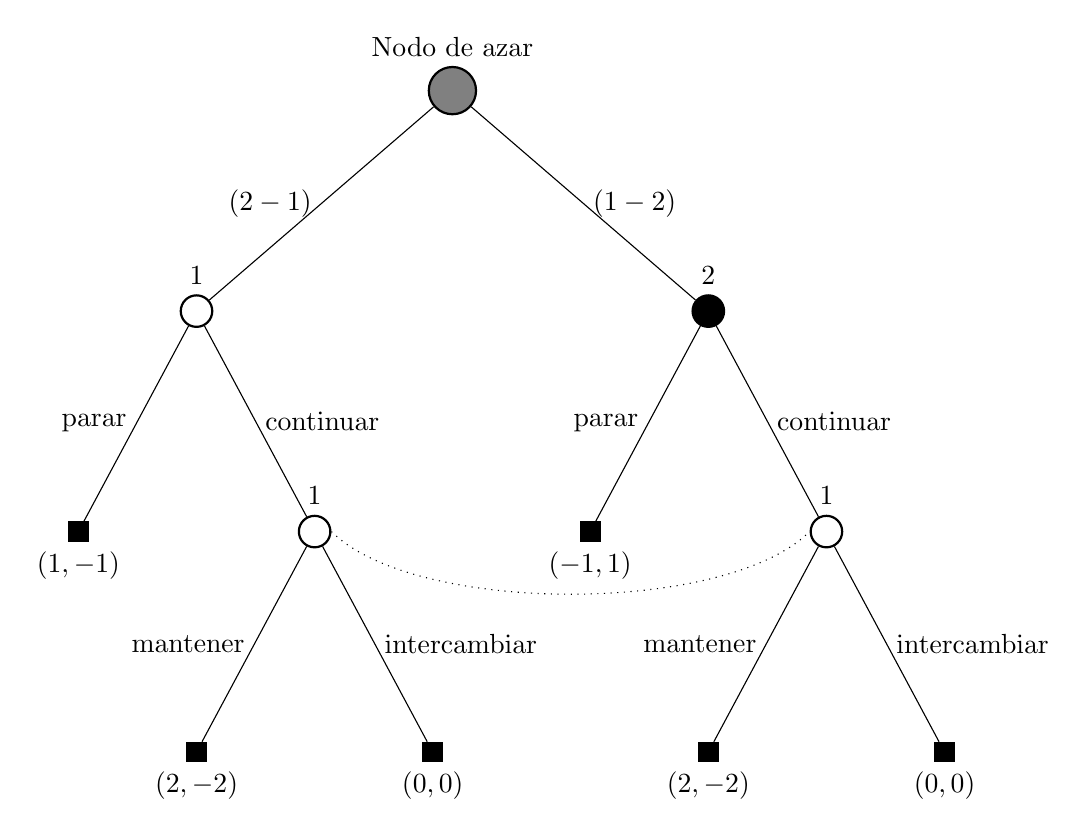
\begin{tikzpicture}[
chance/.style={circle, draw=black, fill=gray, thick, minimum size = 6mm},
player1/.style={circle, draw=black, thick, minimum size = 4mm},
player2/.style={circle, draw=black, fill=black, thick, minimum size=4mm},
terminal/.style={rectangle, draw=black, fill=black, thick, minimum size=2mm},
level 1/.style={sibling distance=65mm, level distance=28mm},
level 2/.style={sibling distance=30mm, level distance=28mm},
level 3/.style={sibling distance=30mm, level distance=28mm},
]

\node[chance] [label = {Nodo de azar}] {}
	child { node[player1] [label=above:{$1$}] {}
    	child { node[terminal] [label=below:{$(1, -1)$}] {} 
        		edge from parent node[left] {parar} }
        child { node (A) [player1] [label=above:{$1$}] {}
        		child { node[terminal] [label=below:{$(2, -2)$}] {}
                		edge from parent node[left] {mantener} }
                child { node[terminal] [label=below:{$(0,  0)$}] {}
                		edge from parent node[right] {intercambiar} }
        		edge from parent node[right] {continuar}
              }
    	edge from parent node[left] {$(2-1)$}
    }
    child{ node[player2] [label=above:{$2$}] {}
    	child { node (C) [terminal] [label=below:{$(-1, 1)$}] {} 
        		edge from parent node[left] {parar} }
        child { node (B) [player1] [label=above:{$1$}] {}
        		child { node[terminal] [label=below:{$(2, -2)$}] {}
                		edge from parent node[left] {mantener} }
                child { node[terminal] [label=below:{$(0,  0)$}] {}
                		edge from parent node[right] {intercambiar} }
        		edge from parent node[right] {continuar}
              }
    	edge from parent node[right] {$(1-2)$}
    };

\draw[dotted] (A.east) .. controls ++(135:-15mm) and ++(45:-15mm) .. (B.west);
\end{tikzpicture}
\end{center}
\end{figure}

Una pregunta de interés es si es posible sustituir una estrategia mixta por una estrategia de comportamiento o viceversa. Para esto, es necesario establecer la definición equivalencia entre estrategias (Definición \ref{def:equivalencia-estrategias}) y alcanzabilidad de una historia bajo una estrategia pura (Definición \ref{def:alcanzabilidad-historia}).

\begin{definition}
\label{def:equivalencia-estrategias}
Dadas dos estrategias $\sigma$ y $\sigma'$, se dice que son equivalentes si la probabilidad de alcanzar cualquier historia terminal es la misma, es decir si $\pi^\sigma(z) = \pi^{\sigma'}(z)$ para todo $z \in Z$.
\end{definition}

\begin{definition}
\label{def:alcanzabilidad-historia}
Sea $s_i \in S_i$ y $I_i \in \mathcal{I}$, diremos que $I_i$ es alcanzable bajo $s_i$ si $\exists h \in H$ tal que $h \in I_i$ y para toda historia $h' \sqsubset h$, con $P(h') = i$, se tiene que $(h', s_i(h'))$ también es prefijo de $h$.  
\end{definition}

Note que la definición anterior puede ser aplicada tanto a perfiles estratégicos como a estrategias para un jugador en particular, utilizando la definición de $\pi^{\sigma}(z)$ correspondiente.

Luego, las preguntas que se desean responder son las siguientes: (i) ?`Dada una estrategia mixta $\sigma^m$, existe una estrategia de comportamiento $\sigma^b$ tal que $\sigma^m$ y $\sigma^b$ son equivalentes? (ii) ?`Dada una estrategia de comportamiento $\sigma^b$ existe una estrategia mixta $\sigma^m$ tal que $\sigma^b$ y $\sigma^m$ son equivalentes?. Los Teoremas \ref{theo:comportamiento-a-mixta} y \ref{theo:mixta-a-comportamiento} ofrecen respuestas a estas interrogantes.

El Teorema \ref{theo:comportamiento-a-mixta} establece lo siguiente: si para cualquier camino de la raíz a un nodo no se atraviesa $2$ veces o más el mismo conjunto de información, entonces para cualquier estrategia de comportamiento existe una estrategia mixta equivalente. Por otra parte, el Teorema \ref{theo:mixta-a-comportamiento} estable que si todos los jugadores tienen \textit{perfect-recall} entonces para toda estrategia mixta existe una estrategia de comportamiento equivalente.

En particular, si se tiene \textit{perfect-recall} entonces ningún camino pasa por el mismo conjunto de información más de una vez y, por lo tanto, para cualquier estrategia de comportamiento también existe una estrategia de comportamiento equivalente. En efecto, las estrategias de comportamiento es una forma compacta de representar las estrategias en este tipo de juegos.

\begin{theorem}
\label{theo:comportamiento-a-mixta}
Dado un juego en forma extensa y un jugador $i$, tal que: si $h' \sqsubset h$ y $P(h') = P(h) = i$, entonces $I(h') \neq I(h)$. Luego, para cualquier estrategia de comportamiento $\sigma^b_i \in B^i$, la estrategia mixta $\sigma^m_i$ dada por:
\begin{alignat}{1}
\sigma^m_i(s_i) := \prod_{I_i \in \mathcal{I}_i} \sigma^b_i(I_i)(s_i(I_i)) \label{eq:comportamiento-a-mixta}
\end{alignat}
es equivalente a la estrategia $\sigma^b_i$.
\end{theorem}

Antes de presentar la demostración, se mostrará un ejemplo de un juego en el que no se cumple la condición del Teorea \ref{theo:comportamiento-a-mixta}, es decir un juego en el que una historia atraviese más de una vez el mismo conjunto de información. En este tipo de juegos se obtiene que el poder expresivo de una estrategia mixta y el de una estrategia de comportamiento no son comparables. El Ejemplo \ref{ex:imperfect-recall-2} \cite[p.~44]{bib:handbook-blai} muestra esta situación.

\begin{example}
\label{ex:imperfect-recall-2}
Considere un juego de dos jugadores tal que:
\begin{alignat}{1}
H = \{ \emptyset, (L), (R), (L,L), (L,R), (R, U), (R, D)\} \\
 P(\emptyset) = P(L) = 1, \ P(R) = 2 \\
 f(L, L) = (1, 0), \ f(L, R) = (100, 100), \ f(R, U) = (5, 1), \ f(R, D) = (2, 2) \\
\mathcal{I}_1 = \{ \{ \emptyset, (L)\} \}, \ \mathcal{I}_2 = \{ \{ R \} \}
\end{alignat}
Este juego de \textit{imperfect
recall} corresponde al árbol de la Figura \ref{fig:imperfect-recall-2}.
\end{example}

\begin{figure}[ht]
\begin{center}
\caption{Árbol de la forma extensiva del juego con \textit{imperfect recall} presentado en el Ejemplo~\ref{ex:imperfect-recall-2}}
\label{fig:imperfect-recall-2}
\begin{tikzpicture}[
chance/.style={circle, draw=black, fill=black, thick, minimum size = 6mm},
player1/.style={circle, draw=black, thick, minimum size = 4mm},
player2/.style={circle, draw=black, fill=black, thick, minimum size=4mm},
terminal/.style={rectangle, draw=black, fill=black, thick, minimum size=2mm},
level 1/.style={sibling distance=60mm, level distance=30mm},
level 2/.style={sibling distance=40mm, level distance=25mm},
]
\node[player1] (A) [label=$1$] {}
	child { node (B) [player1] [label=left:{$1$}]  {}
    	child { node [terminal] [label=below:{$(1,0)$}] {}
        		edge from parent node[left] {$L$} }
        child { node [terminal] [label=below:{$(100,100)$}] {}
        		edge from parent node[right] {$R$} }
        edge from parent node[left] {$L$}
    }
    child { node [player2] [label=right:{$2$}] {}
    	child { node [terminal] [label=below:{$(5,1)$}] {}
        		edge from parent node[left] {$U$} }
        child { node [terminal] [label=below:{$(2,2)$}] {}
        		edge from parent node[right] {$D$} }
        edge from parent node[right] {$R$}
    };
\draw [dotted]
(A.west) .. controls ++(left:+15mm) and ++(90:+15mm) .. (B.north);
\end{tikzpicture}
\end{center}
\end{figure}

Note que, en efecto, la historia $(L)$ atraviesa $2$ veces el único conjunto de información del jugador $1$, este jugador \textit{olvida} si ya hizo la elección entre $L$ o $R$ previamente. En este juego el jugador $1$ tiene $2$ posibles estrategias puras, elegir $L$ o $R$. Por lo tanto, en una estrategia mixta el elige una de estas $2$ acciones según alguna distribución de probabilidad, si embargo, luego de la elección siempre realizará la misma jugada cuando pase por ese conjunto de información. En particular, la historia $(L, R)$ no puede ocurrir y el pago de $100$ es irrelevante en el contexto de estrategias mixtas.

En este juego en particular, se tiene que la estrategia $R$ es mejor para el jugador $1$, independientemente de la elección del jugador $2$ y la estrategia pura $D$ del jugador $2$ es mejor respuesta ante cualquier estrategia de $1$. Luego, el único equilibrio de Nash (de estrategias mixtas) es $(\sigma_1, \sigma_2)$, donde $\sigma_1(L) = 0$, $\sigma_1(R) = 1$, $\sigma_2(D) = 1$ y $\sigma_2(U) = 0$, cuya ganancia es igual a $2$ para ambos jugadores.

Por otra parte, si consideramos estrategias de comportamiento, se debe elegir una distribución $(p, 1-p)$ para elegir $L$ y $R$. En este caso la historia $(L, R)$ tiene una probabilidad de $p(1-p)$ de ser elegida y su pago juega un papel relevante al momento de elegir la estrategia óptima. De esta forma, la estrategia mencionada previamente ya no es un equilibrio en estrategias de comportamientos y se obtiene el equilibrio cuando $p = \frac{98}{198}$ y el jugador $2$ elige $D$.
Note que en el Ejemplo \ref{ex:imperfect-recall-2}, para esta estrategia de comportamiento, no existe una estrategia mixta equivalente, sin embargo, cuando se cumple la condición del Teorema \ref{theo:comportamiento-a-mixta}, sí lo es. La prueba se presenta a continuación.

\begin{proof}
Se quiere probar que para todo $z \in Z$, se tiene que $\pi^{\sigma^m_i}(z) = \pi^{\sigma^b_i}(z)$. 
Para cualquier estrategia se denotará con $\sigma_i(s)$ la probabilidad de elegir la estrategia $s_i$ bajo $\sigma_i$. Además, la probabilidad de elegir una estrategia $s_i$ bajo la estrategia $\sigma^b_i$ es exactamente el lado derecho de la Ecuación \ref{eq:comportamiento-a-mixta}, la cual, por definición es la probabilidad de elegir $s_i$ bajo $\sigma^m_i$. Luego se tiene que $\sigma_i^b(s_i) = \sigma_i^m(s_i)$ para cualquier estrategia pura $s_i \in S_i$.

Por otra parte, como ninguna historia atraviesa más de una vez el mismo conjunto de información, se tiene que para cualquier estrategia $\sigma_i$ (mixta o de comportamiento):

\begin{alignat}{1}
\label{eq:definicion-mixta}
\pi^{\sigma_i}(z) = \sum_{\substack{s_i \in S_i \\  z \text{ es} \text{alcanzable} \\ \text{por } s_i} } \sigma_i(s_i)
\end{alignat}

Luego, $\pi^{\sigma_i^b}(z) = \pi^{\sigma_i^m}(z)$ para todo $z \in Z$, obteniendo el resultado deseado. 
\end{proof}

El Teorema \ref{theo:mixta-a-comportamiento} indica cuando es posible encontrar una estrategia mixta equivalente a una estrategia de comportamiento, lo cual ocurre cuando el juego tiene \textit{perfect recall}.

Antes de presentar el siguiente teorema considere nuevamente el Ejemplo \ref{ex:imperfect-recall}, el cual no tiene \textit{perfect recall}. Las estrategias puras para el jugador $1$ en este juego son: (parar, intercambiar), (parar, mantener), (continuar, intercambiar), (continuar, mantener). Las estrategias puras para el jugador $2$ son: (parar) y (continuar). Luego, la Tabla \ref{table:imperfect-recall} es la tabla correspondiente a la forma normal del juego, la cual incluye sólo la función del pago del jugador $1$, ya que al ser un juego de suma $0$, el pago del jugador $2$ se obtiene trivialmente.

\begin{table}[ht]
\begin{center}
\caption[Tabla de la forma normal para un juego con \textit{imperfect recall}]{Tabla de la forma normal para el Juego \ref{ex:imperfect-recall} con imperfect recall}
\label{table:imperfect-recall}
\begin{tabular}{l  c  c }
\hline
& (parar) & (continuar) \\ \hline
(parar,     mantener)     & $0$ & $-\frac{1}{2}$ \\
(parar,     intercambiar) & $0$ & $ \frac{1}{2}$ \\
(continuar, mantener)     & $ \frac{1}{2}$ & $0$ \\
(continuar, intercambiar) & $-\frac{1}{2}$ & $0$ \\ \hline
\end{tabular}
\end{center}
\end{table}

Note que el pago que proporciona la estrategia (parar, intercambiar) al jugador $1$ es no menor que el pago que le proporciona la estrategia (parar, mantener), sin importar lo que juegue el jugador $2$. Asimismo, para éste jugador, la estrategia (continuar, mantener) es mejor que la estrategia (continuar, intercambiar). Esto puede motivar al jugador $1$ a elegir una estrategia mixta en la que la probabilidad asignada a las estrategias (parar, mantener) y (continuar, intercambiar) sea $0$. Supongamos que la estrategia consiste en elegir las estrategias (parar, intercambiar) y (continuar, mantener) con una probabilidad de $\frac{1}{2}$ cada una. La interrogante planteada es la siguiente ?`Existirá una estrategia de comportamiento equivalente a esta estrategia mixta?

La respuesta a la interrogante es no. Para observarlo, considere una estrategia de comportamiento en la que se elige parar con probabilidad $\alpha$ y mantener con una probabilidad $\beta$. La probabilidad de elegir cada una de las estrategias puras se observa en la Tabla \ref{table:proba-ep}

\begin{table}[ht]
\begin{center}
\caption[Probabilidades de las Estrategias Puras]{Probabilidades de cada estrategia pura dada una estrategia de comportamiento para el jugador $1$ del Ejemplo \ref{ex:imperfect-recall}}
\label{table:proba-ep}
\begin{tabular}{c c c}
\hline
& parar ($\alpha$) & continuar ($1 - \alpha$) \\ \hline
mantener ($\beta$)       & $\alpha\beta$     & $(1-\alpha)\beta$    \\
intercambiar ($1-\beta$) & $\alpha(1-\beta)$ & $(1-\alpha)(1-\beta)$\\ \hline
\end{tabular}
\end{center}
\end{table}

En la estrategia mixta deseada la estrategia pura (parar, mantener) tiene probabilidad $0$, por lo que $\alpha = 0$ o $\beta = 0$ debería ser $0$. Sin embargo, si $\alpha = 0$ la estrategia pura (parar, intercambiar) tiene una probabilidad $0$ de ser elegida y si $\beta = 0$ entonces es imposible elegir la estrategia (continuar, mantener). Luego, no existe una estrategia de comportamiento equivalente a la estrategia mixta deseada. Sin embargo, el Ejemplo \ref{ex:imperfect-recall} no tiene \textit{perfect recall}, el Teorema \ref{theo:mixta-a-comportamiento} enuncia que siempre que se tenga \textit{perfect recall} sí es posible.

\begin{theorem}
\label{theo:mixta-a-comportamiento}
Dado un juego finito de $N$ personas en el que el jugador $i$ tiene ``perfect recall". Entonces, para cada estrategia mixta $\sigma^m_i \in \Delta(S_i)$ del jugador $i$, existe una estrategia de comportamiento $\sigma^b_i \in B^i$, equivalente a $\sigma^m_i$.
\end{theorem}

\begin{proof}
Se denotará por $\pi^{\sigma_i}(I_i, a)$ la probabilidad, bajo $\sigma_i$, que $I_i$ sea alcanzable y se elija la acción $a$. De forma más general se denotará con $\pi^{\sigma_i}(I_i, a_1, a_2, ..., a_k)$ la probabilidad que $I_i$ sea alcanzable y que luego el jugador $i$ elija las acciones $a_1, a_2, ... a_k$. Luego se elige la siguiente estrategia de comportamiento:
\begin{alignat}{1}
\sigma_i^b(I_i)(a)\ &=\ P[\text{se elija}\ a\ \text{bajo}\ \sigma^m_i | I_i\ \text{es alcanzable bajo}\ \sigma^m_i] \\
&=\ \frac{P[I_i\ \text{sea alcanzable bajo}\ \sigma^m_i\ \text{y se elija la opción}\ a\ \text{bajo}\ \sigma^m_i]}{ P[I_i\ \text{es alcanzable bajo}\ \sigma^m_i] } \\
&=\ \frac{\pi^{\sigma^m_i}(I_i, a)}{\pi^{\sigma^m_i}(I_i)} \label{eq:mixta-a-comportamiento}
\end{alignat}

En caso que $\pi^{\sigma^m_i}(I_i) > 0$ y de forma arbitraria en caso contrario.

Se demostrará que $\pi^{\sigma^b_i}(z) = \pi^{\sigma^m_i}(z)$, cuando $\pi^{\sigma^m_i}(z) > 0$. 
	
Dado $z \in Z $, sean $a_1, a_2, ..., a_k$ las acciones elegidas por el jugador $i$ (en ese orden), y sean $I^1_i, I^2_i, ..., I^k_i$ los conjuntos de información respectivos. Note que $\pi^{\sigma^m_i}(I^j_i, a^j_i) = \pi^{\sigma^m_i}(I^{j+1}_i)$, luego:
\begin{alignat}{1}
\pi^{\sigma^b_i}(z)\ &=\ \prod_{j = 1}^k \sigma^b_i(I^j_i)(a^j_i)\ =\ \prod _{j = 1}^k \frac{\pi^{\sigma^m_i}(I^j_i, a_j)}{\pi^{\sigma^m_i}(I^j_i)}\ =\ \frac{\pi^{\sigma^m_i}(I^k_i, a_k)}{\pi^{\sigma^m_i}(I^1_i)}\ =\ \pi^{\sigma^m_i}(I^k_i, a_k)
\end{alignat}

Además, usando inducción, se obtiene que para cualquier $k' < k$ se tiene:
\begin{alignat}{1}
\pi^{\sigma^m_i}(I^k_i, a_k)\ =\ \pi^{\sigma^m_i} (I^{k'}_i, a_{k'}, a_{k'+1}, ..., a_{k})
\end{alignat}

Entonces
\begin{alignat}{1}
\pi^{\sigma^m_i}(I^k_i, a_k) = \pi^{\sigma^m_i}(I^1_i, a_1, a_2, ..., a_k) = \pi^{\sigma^m_i}(z)
\end{alignat}

Obteniendo $\pi^{\sigma^b_i}(z) = \pi^{\sigma^m_i}(z)$, que era lo que se quería demostrar.
\end{proof}

Se puede observar que cuando se tiene un juego con \textit{perfect recall}, se cumplen las condiciones de los Teoremas \ref{theo:mixta-a-comportamiento} y \ref{theo:comportamiento-a-mixta}. Por lo tanto se pueden intercambiar estrategias mixtas por estrategias de comportamiento y viceversa sin perder poder expresivo. Esto se enuncia con el Teorema \ref{theo:equivalencia-estrategias} \cite[p.~45]{bib:handbook-blai}.

\begin{theorem}
\label{theo:equivalencia-estrategias}
En un juego con \textit{perfect recall}, cualquier estrategia mixta de un agente dado puede ser remplazada por una estrategia de comportamiento equivalente, y cualquier estrategia de comportamiento puede ser remplazada por una estrategia mixta equivalente. Dos estrategias son equivalentes en el sentido en que inducen los mismos resultados de probabilidades, para cualquier perfil estratégico fijo (mixto o de comportamiento) del resto de los agentes.
\end{theorem}

Como corolario del teorema anterior se obtiene que el conjunto de los equilibrios de Nash o cambia si el estudio se restringe a estrategias de comportamiento. Los juegos estudiados en este trabajo presentan \textit{perfect recall}, por lo tanto, en las próximas secciones se restringirá el estudio a estrategias de comportamientos. Se asumirá que todas las estrategias son de comportamiento y por lo tanto se denotarán únicamente por $\sigma$ (en vez de $\sigma^b$). Sin embargo, es importante resaltar nuevamente, que esta equivalencia es cierto solamente si el juego tiene \textit{perfect recall}. En juegos generales con información incompleta, estrategias mixtas y de comportamiento mantienen conjuntos de equilibrio no comparables \cite[p.~45]{bib:handbook-blai}.


\section{Equilibrio de Nash en el Juego Kunh Poker}

La descripción del juego se encuentra en la sección \ref{section:kuhn-poker}. Con respecto a la solución, se tiene que el jugador $2$ tiene una ganancia esperada de $\frac{1}{18}$ por mano, como se prueba en \cite{bib:kuhn-poker}, si ambos jugadores juegan de forma óptima (es decir, acorde a un equilibrio de Nash). El equilibrio de Nash se resume en la Tabla \ref{tab:estrategia-kuhn-poker}, donde los conjuntos de información fueron enumerados en un orden de búsqueda por profundidad (dfs).

\begin{table}[ht]
    \centering
    \begin{tabular}{c|r r}
        \hline
        I & \multicolumn{2}{|c}{Equilibrio de Nash}  \\ \hline
         $1$ & $1-\alpha$ & $\alpha$ \\
         $2, 3, 6, 10$ & $1$ & $0$ \\
         $4$ & $\frac{2}{3}$ & $\frac{1}{3}$ \\
         $5, 7, 12$ & $0$ & $1$ \\
         $8$ & $\frac{2}{3}$ & $\frac{1}{3}$ \\
         $9$ & $\frac{2}{3} - \alpha$ & $\alpha + \frac{1}{3}$ \\
        $11$ & $1 - 3 \alpha$ & $3 \alpha$ \\ \hline
    \end{tabular}
    \caption{Equilibrio de Nash para el juego de Kuhn Poker}
    \label{tab:estrategia-kuhn-poker}
\end{table}


El primer jugador tiene infinitas estrategias óptimas, las cuales pueden ser representadas por la elección de un parámetro $\alpha \in [ 0, \frac{1}{3} ]$. Una vez elegido este parámetro, el primer jugador en su primera jugada debe apostar con probabilidad $\alpha$ cuando su carta tenga el número $1$, apuestar con una probabilidad $3 \alpha$ cuando tenga el número $3$ y pasar siempre cuando tenga el número $2$. Si el primer jugador tiene un segundo turno, debe pasar siempre que tenga el número $1$, apostar cuando tiene el número $3$, y en el caso que tenga el número $2$ debe apostar con probabilidad $\alpha + \frac{1}{3}$.

El segundo jugador tiene una única estrategia mixta óptima: apostar siempre que tenga el número $3$. Cuando tenga el número $1$, pasar siempre que el primer jugador haya apostado y apostar con probabilidad $\frac{1}{3}$ en caso contrario. Cuando tenga el número $2$, debe pasar cuando el oponente haya pasado previamente y apostar con probabilidad $\frac{2}{3}$ en caso contrario. La figura \ref{fig:kunh-poker-estrategias} muestra el árbol con las distribuciones de probabilidad de las estrategias previamente descritas en cada uno de los nodos alcanzables en el juego.

\begin{figure}[ht]
\begin{center}
\caption{Equilibrio de Nash del juego de Kunh poker}
\label{fig:kunh-poker-estrategias}
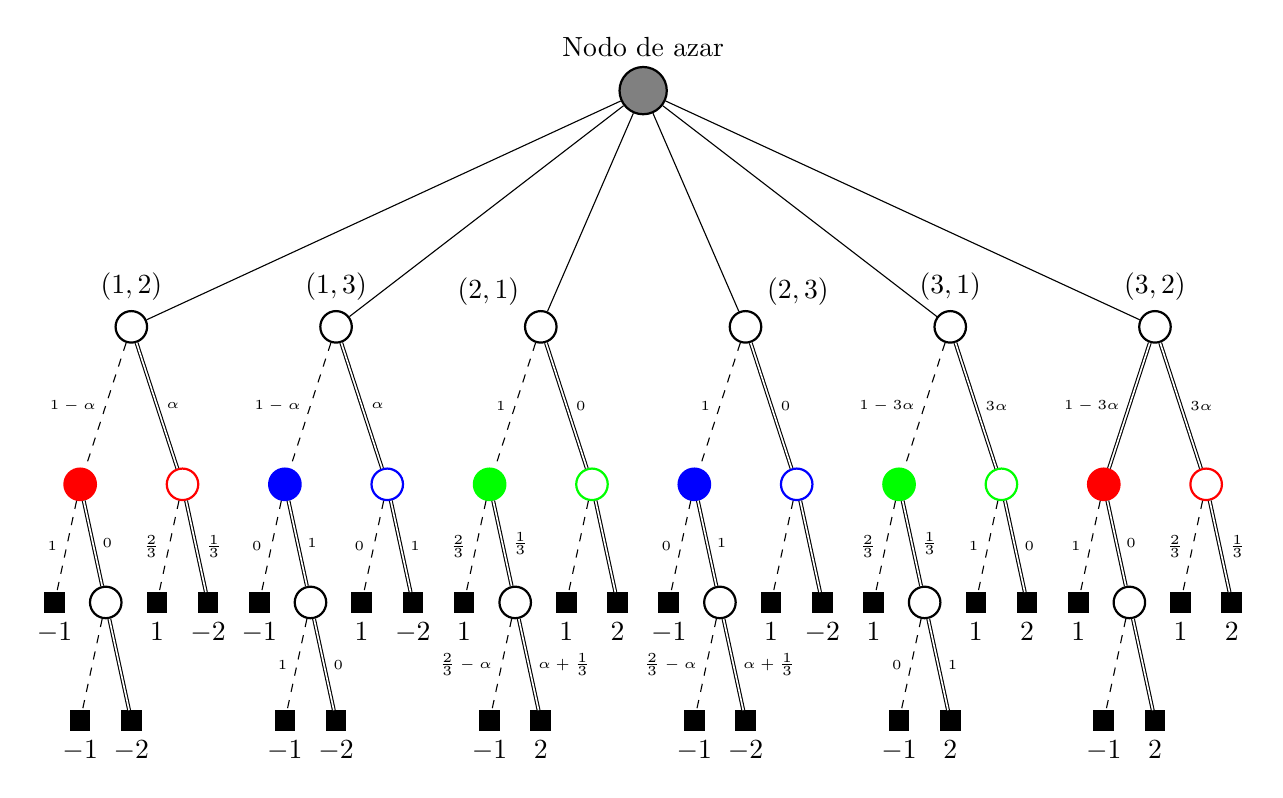
\begin{tikzpicture}[
chance/.style={circle, draw=black, fill=gray, thick, minimum size = 6mm},
player1/.style={circle, draw=black, solid, thick, minimum size = 4mm},
player2/.style={circle, thick, minimum size=4mm},
terminal/.style={rectangle, draw=black, solid, fill=black, thick, minimum size=2mm},
level 1/.style={sibling distance=26mm, level distance=30mm},
level 2/.style={sibling distance=13mm, level distance=20mm},
level 3/.style={sibling distance=6.5mm, level distance=15mm},
]
\node[chance] [label=above:{Nodo de azar}] {} {
	child {node [player1] (P1) [label=above:{$(1, 2)$}]{}
		child { node [player2] [draw=red, fill=red] {} 
				child { node [terminal] [label=below:{$-1$}] {}
						edge from parent [dashed] node [left, draw=none] {\tiny{$1$}} {} }
				child { node [player1] (A) {} 
						child { node [terminal] [label=below:{$-1$}] {}
								edge from parent [dashed] {} }
						child { node [terminal] [label=below:{$-2$}] {} 
								edge from parent [solid, double] {} }
						edge from parent [solid, double] node [right, draw=none] {\tiny{$0$}}  {}
				}
				edge from parent [dashed] node [left, draw=none] {\tiny{$1-\alpha$}}  {}
		}
		child { node [player2] [draw=red] {} 
				child { node [terminal] [label=below:{$1$}] {}
						edge from parent [dashed] node [left, draw=none] {\tiny{$\frac{2}{3}$}} {} }
				child { node [terminal] [label=below:{$-2$}] {}
						edge from parent [solid, double] node [right, draw=none] {\tiny{$\frac{1}{3}$}} {} }
				edge from parent [solid, double] node [right, draw=none] {\tiny{$\alpha$}}{}
		}
	}
	child {node [player1] (P2) [label=above:{$(1, 3)$}]{}
		child { node [player2] [draw=blue, fill=blue] {} 
				child { node [terminal] [label=below:{$-1$}] {}
						edge from parent [dashed] node [left, draw=none] {\tiny{$0$}} {} }
				child { node [player1] (B) {} 
						child { node [terminal] [label=below:{$-1$}] {}
								edge from parent [dashed] node [left, draw=none] {\tiny{$1$}} {} }
						child { node [terminal] [label=below:{$-2$}] {}
								edge from parent [solid, double] node [right, draw=none] {\tiny{$0$}} {} }
						edge from parent [solid, double] node [right, draw=none] {\tiny{$1$}} {}
				}
				edge from parent [dashed] node [left, draw=none] {\tiny{$1-\alpha$}} {}
		}
		child { node [player2] [draw=blue] {} 
				child { node [terminal] [label=below:{$1$}] {}
						edge from parent [dashed] node [left, draw=none] {\tiny{$0$}} {} }
				child { node [terminal] [label=below:{$-2$}] {}
						edge from parent [solid, double] node [right, draw=none] {\tiny{$1$}} {} }
				edge from parent [solid, double] node [right, draw=none] {\tiny{$\alpha$}} {}
		}
	}
	child {node [player1] (P3) [label=135:{$(2, 1)$}]{}
		child { node [player2] [draw=green, fill=green] {} 
				child { node [terminal] [label=below:{$1$}] {}
						edge from parent [dashed] node [left, draw=none] {\tiny{$\frac{2}{3}$}} {} }
				child { node [player1] (C) {} 
						child { node [terminal] [label=below:{$-1$}] {}
								edge from parent [dashed] node [left, draw=none] {\tiny{$\frac{2}{3}-\alpha$}} {} }
						child { node [terminal] [label=below:{$2$}] {} 
                        		edge from parent [solid, double] node [right, draw=none] {\tiny{$\alpha+\frac{1}{3}$}} {} }
						edge from parent [solid, double] node [right, draw=none] {\tiny{$\frac{1}{3}$}} {}
				}
				edge from parent [dashed] node [left, draw=none] {\tiny{$1$}} {}
		}
		child { node [player2] [draw=green] {} 
				child { node [terminal] [label=below:{$1$}] {}
						edge from parent [dashed] {} }
				child { node [terminal] [label=below:{$2$}] {}
						edge from parent [solid, double] {} }
				edge from parent [solid, double] node [right, draw=none] {\tiny{$0$}} {}
		}
	}
	child {node [player1] (P4) [label=45:{$(2, 3)$}]{}
		child { node [player2] [draw=blue, fill=blue]{} 
				child { node [terminal] [label=below:{$-1$}] {}
						edge from parent [dashed] node [left, draw=none] {\tiny{$0$}} {} }
				child { node [player1] (D) {} 
						child { node [terminal] [label=below:{$-1$}] {}
								edge from parent [dashed] node [left, draw=none] {\tiny{$\frac{2}{3}-\alpha$}} {} {} }
						child { node [terminal] [label=below:{$-2$}] {}
								edge from parent [solid, double] {} node [right, draw=none] {\tiny{$\alpha+\frac{1}{3}$}} {} }
						edge from parent [solid, double] node [right, draw=none] {\tiny{$1$}} {}
				}
				edge from parent [dashed] node [left, draw=none] {\tiny{$1$}} {}
		}
		child { node [player2] [draw=blue] {} 
				child { node [terminal] [label=below:{$1$}] {}
						edge from parent [dashed] {} }
				child { node [terminal] [label=below:{$-2$}] {}
						edge from parent [solid, double] {} }
				edge from parent [solid, double] node [right, draw=none] {\tiny{$0$}} {}
		}
	}
	child {node [player1] (P5) [label=above:{$(3, 1)$}]{}
		child { node [player2] [draw=green, fill=green] {} 
				child { node [terminal] [label=below:{$1$}] {}
						edge from parent [dashed] node [left, draw=none] {\tiny{$\frac{2}{3}$}} {} }
				child { node [player1] (E) {} 
						child { node [terminal] [label=below:{$-1$}] {}
								edge from parent [dashed] node [left, draw=none] {\tiny{$0$}} {} }
						child { node [terminal] [label=below:{$2$}] {}
								edge from parent [solid, double] node [right,draw=none] {\tiny{$1$}} {} }
						edge from parent [solid, double] node [right, draw=none] {\tiny{$\frac{1}{3}$}} {}
				}
				edge from parent [dashed] node [left, draw=none] {\tiny{$1-3 \alpha$}} {}
		}
		child { node [player2] [draw=green] {} 
				child { node [terminal] [label=below:{$1$}] {}
						edge from parent [dashed] node [left, draw=none] {\tiny{$1$}} {} }
				child { node [terminal] [label=below:{$2$}] {}
						edge from parent [solid, double] node [right, draw=none] {\tiny{$0$}} {} }
				edge from parent [solid, double] node [right, draw=none] {\tiny{$3 \alpha$}} {}
		}
	}
	child {node [player1] (P6) [label=above:{$(3, 2)$}]{}
		child { node [player2]  [draw=red, fill=red] {} 
				child { node [terminal] [label=below:{$1$}] {}
						edge from parent [dashed] node [left, draw=none] {\tiny{$1$}} {} }
				child { node [player1] (F) {} 
						child { node [terminal] [label=below:{$-1$}] {}
								edge from parent [dashed] {}}
						child { node [terminal] [label=below:{$2$}] {}
								edge from parent [solid, double] {} }
						edge from parent [solid, double] node [right, draw=none] {\tiny{$0$}} {}
				}
				edge from parent [solid, double] node [left, draw=none] {\tiny{$1-3\alpha$}} {}
		}
		child { node [player2]  [draw=red] {} 
				child { node [terminal] [label=below:{$1$}] {}
						edge from parent [dashed] node [left, draw=none] {\tiny{$\frac{2}{3}$}} {} }
				child { node [terminal] [label=below:{$2$}] {}
						edge from parent [solid, double] node [right, draw=none] {\tiny{$\frac{1}{3}$}} {} }
				edge from parent [solid, double] node [right, draw=none] {\tiny{$3\alpha$}} {}
		}
	}
};
\end{tikzpicture}
\end{center}
\end{figure}

\section{Counterfactual Regret Minimization}
\label{section:cfr}

El objetivo de esta sección es presentar un algoritmo que permita encontrar un equilibrio de Nash en un juego en forma extensiva no determinista con información incompleta. Aunque todo juego en forma extensiva puede ser representado en forma normal, esto no es de mucho interés, pues la forma normal puede tener un tamaño exponencialmente más grande al tamaño del árbol. Se verá como el concepto de \textit{regret minimization} puede ser extendido a juegos secuenciales, sin necesidad de la forma normal explícita. Los conceptos, procedimientos y teoremas mostrados en esta sección, son presentados en \cite{bib:cfr}.

\subsection{Regret Minimization}

La primera definición clave es el \textit{regret}. Para esto, es necesario considerar jugar repetidamente un juego en forma extensiva. Sea $\sigma_i^t$ la estrategia usada por el jugador $i$ a tiempo $t$. La Definición \ref{def:average-overall-regret}, presenta el concepto de \textit{average overall regret}.

\begin{definition}
\label{def:average-overall-regret}
El \textbf{average overall regret} del jugador $i$ a tiempo $T$ es:
\begin{alignat}{1}
R_i^T = \frac{1}{T} \max_{\sigma^* in B_i} \sum_{t = 1}^T [u_i(\sigma_i^*, \sigma_{-i}^t) - u_i(\sigma^t)]
\end{alignat}
\end{definition}

Se denotará con $\bar{\sigma}_i^{T}$ la estrategia promedio del jugador $i$ del tiempo $1$ al tiempo $T$. En particular, para cada conjunto de información $I \in \mathcal{I}_i$ y para cada acción $a \in A(I)$ se define:
\begin{alignat}{1}
\bar{\sigma}_i^{T}(I)(a) = \frac{\sum_{t = 1}^T \pi^{\sigma^t_i}(I)\sigma^t_i(I)(a)}{\sum_{t = 1}^T \pi^{\sigma_i^t}(I)}
\end{alignat}

Esta estrategia es el promedio ponderado de las probabilidades $\sigma^t(I)(a)$ con respecto a que tan probable es alcanzar $I$ dado $\sigma_i^t$.

La relación entre el \textit{average overall regret} y el concepto de solución se muestra en el Teorema \ref{theo:regret-nash} \cite{bib:cfr}.
\begin{theorem}
\label{theo:regret-nash}
En un juego de $2$ jugadores de suma cero si el average overall regret a tiempo $T$ es menor que $\varepsilon$ entonces $\sigma^{-T}$ es un $2\varepsilon$-equilibrio de Nash
\end{theorem}
\begin{proof}

Se probará que la probabilidad de alcanzar $z$ bajo $\bar{\sigma}_i^T$ viene dada por el promedio de alcanzar $z$ en cada estrategia. Sean $h_1 \sqsubset h_2 \sqsubset h_3 \sqsubset ... \sqsubset h_m \sqsubset z$ todos los prefijos de $z$ correspondientes al jugador $i$, es decir $P(h_k) = i\ \forall k : 1 \leq k \leq m$ y sean $a_1, a_2, ..., a_m$ las acciones correspondientes en $z$ en cada historia respectiva. Luego:
\begin{alignat}{2}
\pi^{\bar{\sigma}_i^T}(z)\ &=\ \prod_{k = 1}^m \bar{\sigma}_i^T(I(h_k))(a_k) \\	&=\ \prod_{k = 1}^m \frac{\sum_{t = 1}^{T}  \pi^{\sigma_i^t}(I(h_k))\sigma^t_i(I(h_k))(a)}{\sum_{t = 1}^T \pi^{\sigma_i^t}(I(h_k))}
\end{alignat}

Por otra parte, note que $\pi^{\sigma_i^t}(I)\sigma_i^t(I(h_k))(a_k) = \pi^{\sigma_i^t}(I(h_{k+1}))$. Entonces:
\begin{alignat}{1}
	\pi^{\bar{\sigma}_i^T}(z)\ &=\ \frac{\sum_{t = 1}^T\pi^{\sigma_i^t}(I_m) \sigma_i^t(I_m)(a_m)}{\sum_{t = 1}^T \pi^{\sigma_i^t}(I_1)} \\
	&=\ \frac{\sum_{t = 1}^T \pi^{\sigma_i^t}(z)}{\sum_{t = 1}^T 1} \\
	&=\ \frac{1}{T} \sum_{t = 1}^T \pi^{\sigma_i^t}(z)
\end{alignat}

Además, se tiene que, para cualquier jugador $i$ y cualquier estrategia de $\sigma_i$:
\begin{alignat}{2}
\frac{1}{T} \sum_{t = 1}^T u_i(\sigma'_i, \sigma_{-i}^t)\ &=\ \frac{1}{T} \sum_{t = 1}^T \left( \sum_{z \in Z} \pi^{\sigma'_i}(z) \pi^{\sigma_{-i}^t}(z) \pi^c(z) \right) \\
	&=\ \sum_{z \in Z} u_i(z) \pi^{\sigma'_i}(z) \pi^c(z) \left( \frac{1}{T} \sum_{t = 1}^T \pi^{\sigma_{-i}^t}(z) \right) \\
	&=\ \sum_{z \in Z} u_i(z) \pi^{\sigma'_i}(z) \pi^{\bar{\sigma}_i^T}(z) \pi^c(z) \\
	&=\ u_i(\sigma'_i, \bar{\sigma}_{-i}^T)
\end{alignat}

Por otra parte, como $R_2^T \leq \varepsilon$, para todo $\sigma'_2 \in B_2$ se tiene que:
\begin{alignat}{2}
	& \frac{1}{T} \sum_{t = 1}^T[u_2(\sigma_1^t, \sigma'_2) - u_2(\sigma^t)]\  \leq\  \varepsilon\\
	\Rightarrow\ & \frac{1}{T} \sum_{t = 1}^T u_2(\sigma^t) + \varepsilon\  \geq\  \frac{1}{T} \sum_{t = 1}^T u_2(\sigma_1^t, \sigma'_2) \\
	\Rightarrow\ & \frac{1}{T} \sum_{t = 1}^T u_2(\sigma^t) + \varepsilon\ \geq\ u_2(\bar{\sigma}_1^T, \sigma'_2)
\end{alignat}

Luego, como se cumple para cualquier $\sigma'_2$, se cumple para $\sigma_2^t$ para $t = 1, 2, ..., T$, obteniendo:
\begin{alignat}{2}
\frac{1}{T} \sum_{t = 1}^T u_2(\sigma^t) + \varepsilon\ & \geq\ \frac{1}{T} \sum_{t = 1}^T u_2(\bar{\sigma}_1^T, \sigma_2^t) \\
&=\ \frac{1}{T} \sum_{t = 1}^T \sum_{z \in Z} u_2(z) \pi^{\bar{\sigma}_1^T}\pi^{\sigma_2^t}(z) \pi^c(z) \\
&=\  \sum_{z \in Z} u_2(z) \pi^{\bar{\sigma}_1^T} \pi^c(z) \left( \frac{1}{T} \sum_{t = 1}^T \pi^{\sigma_2^t}(z) \right)\\
&=\  \sum_{z \in Z} u_2(z) \pi^{\bar{\sigma}_1^T} \pi^{\bar{\sigma}_2^T} \pi^c(z) \\
&=\ u_2(\bar{\sigma}^T)
\end{alignat}

Como $\Gamma$ es un juego de suma cero, se tiene que $u_2 = -u_1(\sigma)$ para toda estrategia $\sigma$, luego:
\begin{alignat}{2}
	& \frac{1}{T} \sum_{t = 1}^T u_2(\sigma^t) + \varepsilon\ \geq\  u_2(\bar{\sigma}^T) \\
	\Rightarrow\ & \frac{1}{T} \sum_{t = 1}^T -u_1(\sigma^t) + \varepsilon\ \geq\  -u_1(\bar{\sigma}^T) \\
	\Rightarrow\ &  u_1(\bar{\sigma}^T)\ + \varepsilon\ \geq\   \frac{1}{T} \sum_{t = 1}^T u_1(\sigma^t)  \\
	\Rightarrow\ &  u_1(\bar{\sigma}^T)\ + 2\varepsilon\ \geq\   \frac{1}{T} \sum_{t = 1}^T u_1(\sigma^t) + \varepsilon
\end{alignat}

Por otra parte, como $R_i^t \leq \varepsilon$ se tiene que, para cualquier $\sigma'_1 \in B_1$:
\begin{alignat}{1}
	\frac{1}{T} \sum_{t = 1}^T u_1(\sigma^t) + \varepsilon\ \geq\ \frac{1}{T} \sum_{t = 1} u_1(\sigma'_1, \sigma_2^t)\ =\ u_1(\sigma'_1, \bar{\sigma}_2^T)
\end{alignat}

Luego, se obtiene que:
\begin{alignat}{1}
	& u_1(\bar{\sigma}^T)\ + 2\varepsilon\ \geq\   \frac{1}{T} \sum_{t = 1}^T u_1(\sigma^t) + \varepsilon\ \geq\ u_1(\sigma'_1, \bar{\sigma}_2^T)\\
	\Rightarrow\ & u_1(\bar{\sigma}^T)\ + 2\varepsilon\ \geq\ u_1(\sigma'_1, \bar{\sigma}_2^T)
\end{alignat}

Análogamente, se demuestra que:
\begin{alignat}{1}
	u_2(\bar{\sigma}^T)\ + 2\varepsilon\ \geq\ u_2( \bar{\sigma}_1^T, \sigma'_2)
\end{alignat}

Concluyendo que $\bar{\sigma}^T$ es un $2\varepsilon$-equilibrio correlacionado.
\end{proof}

Como consecuencia del teorema anterior se obtiene que un algoritmo que lleve el \textit{average overall regret} a cero, conducirá a un equilibrio de Nash. La idea fundamental del enfoque presentado a continuación, propuesto en \cite{bib:cfr}, consiste en descomponer el \textit{average overall regret} en un conjunto de términos aditivos de \textit{regret} que puedan ser minimizados independientemente. En particular es necesario introducir un par de nuevo concepto, la utilidad contrafactual (Definición \ref{def:utilidad-contrafactual}) y el \textit{regret} contrafactual inmediato (Definición \ref{def:regret-inmediato}).

\begin{definition}
\label{def:utilidad-contrafactual}
La \textbf{utilidad contrafactual} es la ganancia esperada dado que el conjunto $I$ es alcanzado y todos los jugadores juegan con la estrategia $\sigma$ con excepción del jugador $i$ que juega para alcanzar $I$. Formalmente, si $\pi^{\sigma}(h, h')$ es la probabilidad de ir de la historia $h$ a la historia $h'$, entonces:
\begin{alignat}{1}
u_i(\sigma, I) = \frac{\sum_{h \in I, z \in Z} \pi^{\sigma_{-i}(h)} \pi^{\sigma}(h, z) u_i(z)}{\pi^{\sigma_{-i}}(I)}
\end{alignat}
\end{definition}

Para toda acción $a \in A(I)$, se define $\sigma|_{I \rightarrow a}$ como el perfil estratégico idéntico a $\sigma$ excepto que el jugador $i$ siempre elige $a$ en el conjunto de información $I$.

\begin{definition}
\label{def:regret-inmediato}
El \textbf{regret contrafactual inmediato} es:
\begin{alignat}{1}
R_{i, \text{imm}}^T (I) = \frac{1}{T} \max_{a \in A(I)} \sum_{t = 1}^T \pi^{\sigma_{-i}^t}(I)[u_i(\sigma^t|_{I \rightarrow a}, I) - u_i(\sigma^t, I)]
\end{alignat}
\end{definition}

Intuitivamente, el \textit{regret} contrafactual inmediato es el arrepentimiento del jugador $i$ en su decisión en el conjunto de información $I$, en términos de la utilidad contrafactual, con un término de ponderación adicional para la probabilidad contrafactual que $I$ alcanzaría en esa ronda si el jugador hubiera intentado hacer eso. Usualmente, es de mayor interés el \textit{regret} cuando es positivo, por lo que se define $R_{i, \text{imm}}^{T, +} (I) = max(R^T_{i, \text{imm}} (I), 0)$. Luego, se tiene el siguiente resultado:

\begin{theorem}
\begin{alignat}{1}
R_i^T \leq \sum_{I \in \mathcal{I}_i} R_{i, \text{imm}}^{T, +}(I)
\end{alignat}
\end{theorem}

Debido a que minimizar cada \textit{regret} contrafactual inmediato minimiza el \textit{average overall regret} arrepentimiento general promedio, es posible enfocarse en minimizar los primeros para obtener un equilibrio de Nash.

\subsection{Counterfactual Regret Minimization}

Antes de mostrar el algoritmo principal, denominado \textit{Counterfactual Regret Minimization} para los juegos en forma extensiva, es necesario introducir el algoritmo de \textit{Regret Matching} general. Este algoritmo puede ser descrito en un dominio donde hay un conjunto fijo de acciones $A$, una función $u^t : A \rightarrow \mathbb{R}$ y en cada ronda una distribución de probabilidad $p^t$ es elegida.

\begin{definition}
\label{def:regret}
El \textit{regret} de no haber elegido la acción $a \in A$ hasta tiempo $T$, se define como:
\begin{alignat}{1}
R_i^T(a) = \frac{1}{T} \sum_{t = 1}^T \left[u_i(a) - \sum_{a' \in A}p^t(a)u^t(a)\right]
\end{alignat}
\end{definition}

Se define $R^{t, +}(a) = \max(R^t(a), 0)$. Luego la distribución $p^{t+1}$ es elegida de la siguiente manera:
\begin{alignat}{1}
p^t(a) = 
\begin{cases}
\frac{R_i^{t, +}}{\sum_{a' \in A} R^{t, +}(a)}\ & \text{si }\ \sum_{a' \in A} R^{t, +}(a) > 0\\
\frac{1}{|A|}\ & \text{en otro caso}
\end{cases}
\end{alignat}

\begin{theorem}
Si $|u| = \max_{t \in \{1, 2, ... T\}} \max_{a, a' \in A}(u^t(a) - u^t(a'))$ entonces el regret del algoritmo de regret matching está acotado por:
\begin{alignat}{1}
max_{a \in A}R^t(a) \leq \frac{|u| \sqrt{|A|}}{\sqrt T}
\end{alignat}
\end{theorem}

Luego, el algoritmo de \textit{Counterfactual Regret Minimization} es una aplicación del algoritmo \textit{Regret Minimization} de forma independiente a cada conjunto de información. En particular, se mantiene, para cada $I \in \mathcal{I}_i$ y para todo $a \in A(I)$:
\begin{alignat}{1}
R_i^T(I, a) = \frac{1}{T} \sum_{t = 1}^T \pi^{\sigma^t_{-i}}(I)[u_i(\sigma^t|_{I \rightarrow a}, I) - u_i(\sigma^t, I)]
\end{alignat}

Se define $R_i^{T, +}(I, a) = \max(R_i^T(I, a), 0)$, luego a tiempo $T+1$ la estrategia elegida es:
\begin{alignat}{1}
\sigma_i^{T+1}(I)(a) =
\begin{cases}
\frac{R_i^{T, +}(I, a)}{\sum_{a' \in A(I) R_i^{T, +}(I, a')}}\ & \text{si } \sum_{a' \in A(I) R_i^{T, +}(I, a')} > 0 \\
\frac{1}{|A(I)|}\ & \text{en otro caso} 
\end{cases}
\end{alignat}

Este algoritmo consiste en seleccionar las acciones de forma proporcional a la cantidad del \textit{regret} contrafactual positivo de no haber elegido esa acción. Si ninguna de estas cantidades es positiva, entonces la acción se elige con una distribución uniforme. Luego, como cota de convergencia, se tiene el siguiente teorema:
\begin{theorem}
Si el jugador $i$ selecciona las acciones de acuerdo al procedimiento anterior, entonces $R^T_{i, \text{imm}}(I) \leq \Delta_{u, i} \frac{\sqrt{|A_i|}}{\sqrt{T}}$ y por lo tanto $R_i^T \leq \Delta_{u, i} |\mathcal{I}_i| \frac{|A_i|}{\sqrt T}$, donde $|A_i| = max_{h : P(h) = 1}{|A(h)|}$
\end{theorem}